\chapter{Modell}
\label{ch:model}

\section{Tensoren}
In der Literatur zur Funktionsweise künstlicher neuronaler Netze wird ausnahmlos auch der Begriff Tensor verwendet. Ein Tensor ist ein vielgestaltiges mathematisches Konstrukt. Beispielsweise sind Vektoren und Matrizen Tensoren. In ``Deep Learning with Python'' \cite{chollet2021deep} findet sich die folgende Beschreibung:

Mehrdimensionale Arrays, in NumPy ndarray (N-Dimensional Array) genannt, werden auch Tensoren genannt. Generell verwenden alle derzeitigen Systeme für Maschinelles Lernen Tensoren als zugrundeliegende Datenstruktur. Tensoren sind elementar für dieses Fachgebiet.

In seinem Kern ist ein Tensor ein Container für numerische Daten. Tensoren sind die Verallgemeinerung der Matrizen für eine beliebige Anzahl Dimensionen. Im Zusammenhang mit Tensoren werden die Dimensionen häufig Achsen gennannt. Die Anzahl der Achsen wird auch als Stufe bezeichnet. Ein Skalar ist ein Tensor nullter Stufe. Ein Vektor ist ein Tensor erster Stufe und eine Matrix ein Tensor zweiter Stufe.

Ein Tensor ist durch drei Schlüsselattribute definiert:
\begin{itemize}
\item Anzahl der Achsen (Stufe): Zum Beispiel hat ein Tensor dritter Stufe drei Achsen, und eine Matrix hat zwei Achsen. In Python-Bibliotheken wie NumPy oder Tensorflow wird sie auch als $ndim$ des Tensors bezeichnet.
\item Form: Dies ist ein Tupel aus Ganzzahlen, das die Dimension jeder Achse beschreibt. Beispiele sind $(3, 5)$ für die Form einer Matrix und $(3, 3, 5)$ für einen Tensor dritter Stufe. Ein Vektor hat eine Form mit einem einzelnen Element, etwa so: $(5,)$, während ein Skalar eine leere Form hat: $()$.
\item Datentyp (in Python-Bibliotheken gewöhnlich $dtype$ genannt): Dies ist der Typ der im Tensor enthaltenen Daten. Zum Beispiel könnte der Datentyp eines Tensors $float16$, $float32$, $float64$, $uint8$ und so weiter sein.
\end{itemize}
\cite{chollet2021deep}

Bilder erscheinen als Tensoren dritter Stufe, deren Achsen der Höhe, Breite und den Farbkanälen (Rot, Grün und Blau) entsprechen. \cite{zhang2020dive}

Viele in dieser Arbeit verwendeten Tensoren beschreiben RGB-Bilddaten. Sie sind deshalb dritter Stufe, und die enthaltenen Daten sind Ganzzahlen zwischen $0$ und $255$. Die Form der durch das künstliche neuronale Netz generierten Bilder ist $(256, 256, 3)$. Die Dimensionen beschreiben hier also die Breite, Höhe und Farbtiefe der Bilddateien.

\section{Kreuzentropie}
Kreuzentropie ist ein Begriff aus der Wahrscheinlichkeitsrechnung. In dem Buch Deep Learning von Ian Goodfellow et al. \cite{goodfellow2016deeplearning} wird auf Wahrscheinlichkeitsrechnung wie folgt eingegangen:

In Anwendungen mit künstlicher Intelligenz wird Wahrscheinlichkeitsrechnung auf zwei wesentliche Arten verwendet. Erstens erklären die Regeln der Wahrscheinlichkeit, wie KI-Systeme urteilen sollten, deshalb werden Algorithmen so gestaltet, dass sie vielfältige Ausdrücke mittels Probabilistik berechnen oder annähern. Zweitens können Wahrscheinlichkeitsrechnung und Statistik das Verhalten zu planender KI-Systeme theoretisch analysieren.

Es gibt drei mögliche Quellen von Unsicherheit:

\begin{enumerate}

\item Die dem modellierten System innewohnende Zufälligkeit. Zum Beispiel beschreiben die meisten Interpretationen der Quantenmechanik die Dynamik der subatomaren Partikel als probabilistisch. Es können auch theoretische Szenarios mit zufälligen Dynamiken gebildet werden, wie ein hypothetisches Kartenspiel, in dem die Karten wirklich in einer zufällilgen Reihenfolge gemischt werden.

\item Unvollständige Beobachtbarkeit. Auch deterministische Systeme können stochastisch anmuten, wenn nicht alle Variablen, die das Verhalten des Systems bestimmen, beobachtbar sind. Zum Beispiel, im Monty-Hall-Problem (Ziegenproblem), wird ein Kandidat einer Spielshow aufgefordert, zwischen drei Toren zu wählen und gewinnt einen Preis, der sich hinter der gewählten Tür befindet. Zwei Tore führen zu einer Ziege, während ein drittes zu einem Auto führt. Das Ergebnis aufgrund der Wahl des Kandidaten ist deterministisch, aber aus Sicht des Kandidaten ist das Ergebnis unsicher.

\item Unvollständige Modellierung. Wenn ein Modell einen Teil der beobachteten Informationen verwerfen muss, resultieren die verworfenen Informationen in Unsicherheit bei den Vorhersagen des Modells. Nehmen wir zum Beispiel an, ein Roboter kann die genaue Position jedes Objektes um ihn herum feststellen. Wenn der Roboter den Raum zum Vorhersagen der zukünftigen Position dieser Objekte diskretisiert, dann lässt diese Diskretisierung den Roboter über die präzise Position von Objekten unmittelbar unsicher werden: Jedes Objekt könnte irgendwo innerhalb der diskreten Zelle sein, in der es festgellt wurde.

\end{enumerate}

In vielen Fällen ist es praktikabler, eine einfache aber unsichere Regel statt einer komplexen aber sicheren zu verwenden, selbst wenn die wahre Regel deterministisch ist und ein Modellierungssystem die Genauigkeit besitzt, eine komplexe Regel bereitstellen zu können.

Zum Beispiel ist die einfache Regel ``Die meisten Vögel fliegen'' einfach zu entwickeln und weitgehend nützlich, während eine Regel in der Form ``Vögel fliegen, außer sehr junge Vögel, die noch nicht gelernt haben zu fliegen, kranke und verletzte Vögel, die ihre Fähigkeit zu fliegen verloren haben, flugunfähige Vögel, einschließlich Kasuare, Strauße und Kiwis\dots'' ist aufwändig zu entwickeln, zu warten und zu kommunizieren und nach all dem Aufwand immer noch fragil und fehleranfällig.

Obwohl es naheliegend ist, dass Möglichkeiten Unsicherheit darzustellen und zu diskutieren notwendig sind, ist es nicht sofort offensichtlich, dass die Wahrscheinlichkeitsrechnung alle Werkzeuge für Anwendungen künstlicher Intelligenz bereitstellt.

Wahrscheinlichkeitsrechnung wurde ursprünglich entwickelt, um die Häufigkeit von Ereignissen zu analysieren. Es ist leicht erkennenbar, wie Wahrscheinlichkeitsrechnung verwendet werden kann, um Ereignisse wie das Ziehen einer bestimmten Hand in einem Pokerspiel zu studieren. Diese Art von Ereignissen sind oft wiederkehrend.

Wenn ein Ergebnis die Wahrscheinlichkeit $p$ hat einzutreten, heißt das, dass wenn das Experiment (z.B. eine Hand Karten ziehen) unendlich oft wiederholt würde, dann hätten die Wiederholungen zu dem Anteil $p$ dieses Ergebnis zur Folge.

Dieser Denkansatz scheint auf Vorhaben, die nicht wiederholbar sind, nicht anwendbar zu sein. Wenn ein Arzt seinen Patienten analysiert und feststellt, dass der Patient eine 40\=/prozentige Chance besitzt die Grippe zu haben, heißt das etwas sehr unterschiedliches -- der Patient kann nicht unendlich oft repliziert werden, und es gibt keinen Grund zur Annahme, dass unterschiedliche Replikas des Patienten die gleichen Symptome zeigen, aber unterschiedliche zugrundeliegende Krankheiten haben.

In dem Fall des Arztes, der den Patient diagnostiziert, steht Wahrscheinlichkeit für den Grad der Vermutung, wobei mit $1$ absolute Sicherheit, dass der Patient die Grippe hat, angegeben wird und mit $0$ absolute Sicherheit, dass der Patient die Grippe nicht hat.

Die vorherige Art von Wahrscheinlichkeit, direkt verbunden mit der Häufigkeit, in der Ereignisse eintreten, ist als frequentistische Wahrscheinlichkeit bekannt, während die zweite Art, verbunden mit dem qualitativen Grad der Sicherheit, bekannt ist als Bayessche Wahrscheinlichkeit.
\cite{goodfellow2016deeplearning}

Das Buch Dive into Deep Learning von Aston Zhang et al. \cite{zhang2020dive} nähert sich der Kreuzentropie wie folgt:

Um die Ausgaben als Wahrscheinlichkeiten interpretieren zu können, muss (auch für neue Daten) garantiert sein, dass sie nicht-negativ sind und sich zu $1$ addieren. Weiterhin brauchen wir ein Trainingsziel, das das Modell darin unterstützt genaue Wahrscheinlichkeiten zu schätzen. In allen Fällen sollten, wenn ein Classifier $0.5$ ausgibt, die Hälfte dieser Beispiele tatsächlich zu der vorherberechneten Klasse gehören.

Es wird eine Verlustfunktion benötigt, um die Qualität der vorherberechneten Wahrscheinlichkeiten zu messen. Die Softmax-Funktion gibt einen Vektor $\hat{y}$ aus, der als die geschätzte bedingte Wahrscheinlichkeit jeder Klasse für die gegebene Eingabe $x$ interpretiert werden kann, zum Beispiel $\hat{y}_{1}\ =\ P(y\ =\ cat\ |\ \boldsymbol{x})$.

Angenommen, das gesamte Dataset $\{\boldsymbol{X}, \boldsymbol{Y}\}$ enthält $n$ Beispiele, wobei das Beispiel mit dem Index $i$ aus einem Featurevektor $\boldsymbol{x}^{(i)}$ und einem One-Hot-Label-Vektor $\boldsymbol{y}^{(i)}$ besteht. Die Schätzungen können mit der Wirklichkeit verglichen werden, indem überprüft wird, wie wahrscheinlich die tatsächliche Klasse für die gegebenen Features gemäß dem Modell ist:

\begin{align}
  P(\boldsymbol{Y}\ |\ \boldsymbol{X})\ =\ \prod_{i=1}^{n}P(\boldsymbol{y}^{(i)}\ |\ \boldsymbol{x}^{(i)}).
\end{align}

Entsprechend der Maximum-Likelihood-Methode wird $P(\boldsymbol{Y}\ |\ \boldsymbol{X})$ maximiert, was equivalent zur Minimierung des negativen Log-Likelihood ist:

\begin{align}
  -\log P(\boldsymbol{Y}\ |\ \boldsymbol{X})\ =\ \sum_{i=1}^{n}-\log P(\boldsymbol{y}^{(i)}\ |\ \boldsymbol{x}^{(i)})\ =\ \sum_{i=1}^{n}l(\boldsymbol{y}^{(i)},\boldsymbol{\hat{y}}^{(i)}),
\end{align}

wobei für jedes Paar von Label $\boldsymbol{y}$ und Vorhersage des Modells $\boldsymbol{\hat{y}}$ über $q$ Klassen die Verlustfunktion $l$

\begin{align}
  \label{eq:fn_crossentropy}
  l(\boldsymbol{y}, \boldsymbol{\hat{y}})\ =\ - \sum_{j=1}^{q}y_{j}\log\hat{y}_{j}
\end{align}

ist. Die Verlustfunktion in \eqref{eq:fn_crossentropy} wird gemeinhin als Cross-Entropy-Verlustfunktion bezeichnet. Da $\boldsymbol{y}$ ein One-Hot-Vektor der Länge $q$ ist, verschwindet die Summe über alle seine Koordinaten $j$, bis auf einen Term. Da alle $\hat{y}_j$ vorherberechnete Wahrscheinlichkeiten sind, ist deren Logarithmus niemals größer als $0$. Folglich kann die Verlustfunktion nicht weiter minimiert werden, wenn das tatsächliche Label mit \textit{Sicherheit}, das heißt wenn die vorhergesagte Wahrscheinlichkeit $P(\boldsymbol{y}\ |\ \boldsymbol{x}) = 1$, korrekt vorhergesagt wird.

Nehmen wir nun an, dass wir nicht nur ein einziges Ergebnis, sondern eine ganze Verteilung über Ergebnisse beobachten. Wir können dieselbe Darstellung nutzen wie bisher. Der einzige Unterschied ist, dass statt einem Vektor nur aus binären Einträgen wie zum Beispiel $(0, 0, 1)$ jetzt ein allgemeiner Wahrscheinlichkeitsvektor wie zum Beispiel $(0.1, 0.2, 0.7)$ vorliegt. Die bisher verwendete Mathematik um den Versult zu definieren funktioniert noch genauso gut, nur ist die Interpretation etwas allgemeiner. Es ist der Erwartungswert des Verlustes für eine Verteilung über Labels. Dieser Verlust wird Cross-Entropy-Verlust genannt und es eine der meistverbreitet eingesetzten Verlustfunktionen für Klassifizierungsaufgaben.

Hier ist ein kurzes Beispiel für die Anwendung der Kreuzentropie. Es sei $P$ ein wahre Verteilung mit der Wahrscheinlichkeitsverteilung $p(x)$ und $Q$ die geschätzte Verteilung mit der Wahrscheinlichkeitsverteilung $q(x)$. Angenommen eine Klassifizierungsaufgabe basierend auf $n$ gegebenen Datenbeispielen $\{x_{1}, \dots, x_{n}\}$. Angenommen die positiven und negativen Klassenlabel $y_{i}$ sind als $1$ beziehungsweise $0$ kodiert und ein künstliches neuronales Netz ist parametrisiert durch $\theta$. Wenn es das Ziel ist, das beste $\theta$ zu finden, damit $\hat{y}_{i} = p_{\theta}(y_{i}\ |\ x_{i})$, kann naturgemäß die Maximum-Likelihood-Methode angewendet werden. Konkret ist für die wahren Label $y_{i}$ und die Vorhersagen $\hat{y}_{i} = p_{\theta}(y_{i}\ |\ x_{i})$ die Wahrscheinlichkeit als positiv klassifiziert zu werden $\pi_{i} = p_{\theta}(y_{i} = 1\ |\ x_{i})$.

Daher wäre die Log-Likelihood-Funktion

\begin{align}
  l(\theta)\ &=\ \log L(\theta) \\
  &=\ \log\prod_{i=1}^{n}\pi_{i}^{y_{i}} (1\ -\ \pi_{i})^{1-y_{i}} \tag*{}\\
  &=\ \sum_{i=1}^{n}y_{i}\log(\pi_{i})\ +\ (1\ -\ y_{i})\log(1\ - \pi_{i}). \tag*{}
\end{align}

Die Log-Likelihood-Funktion zu maximieren ist identisch mit dem Minimieren von $-l(\theta)$, und daher kann hiermit der beste Wert für $\theta$ gefunden werden.
\cite{zhang2020dive}

\section{Logistische Regression}
\label{sec:logreg}
Ein vergleichsweise einfacher Algorithmus des Maschinellen Lernens ist Logistic Regression oder Softmax Regression. Es lassen sich damit Klassifizierungen durchführen. Bei binären Klassifizierungen werden die Eingaben in zwei Kategorien unterteilt. Häufige Beispiele sind fehlerfreie oder fehlerhafte Produktionsergebnisse, ärztliche Befunde einer bestimmten Krankheit oder Gesundheit und ob in einem Bild ein bestimmtes Objekt vorhanden ist oder nicht.

Bei der Multiclass Logistic Regression werden die Eingaben in mehr als zwei Klassen unterteilt. Es lassen sich damit beispielsweise in einem Bild  verschiedene Arten von Fahrzeugen, Gegenständen oder Tieren unterteilen.

\begin{figure}[h]
	\centering
	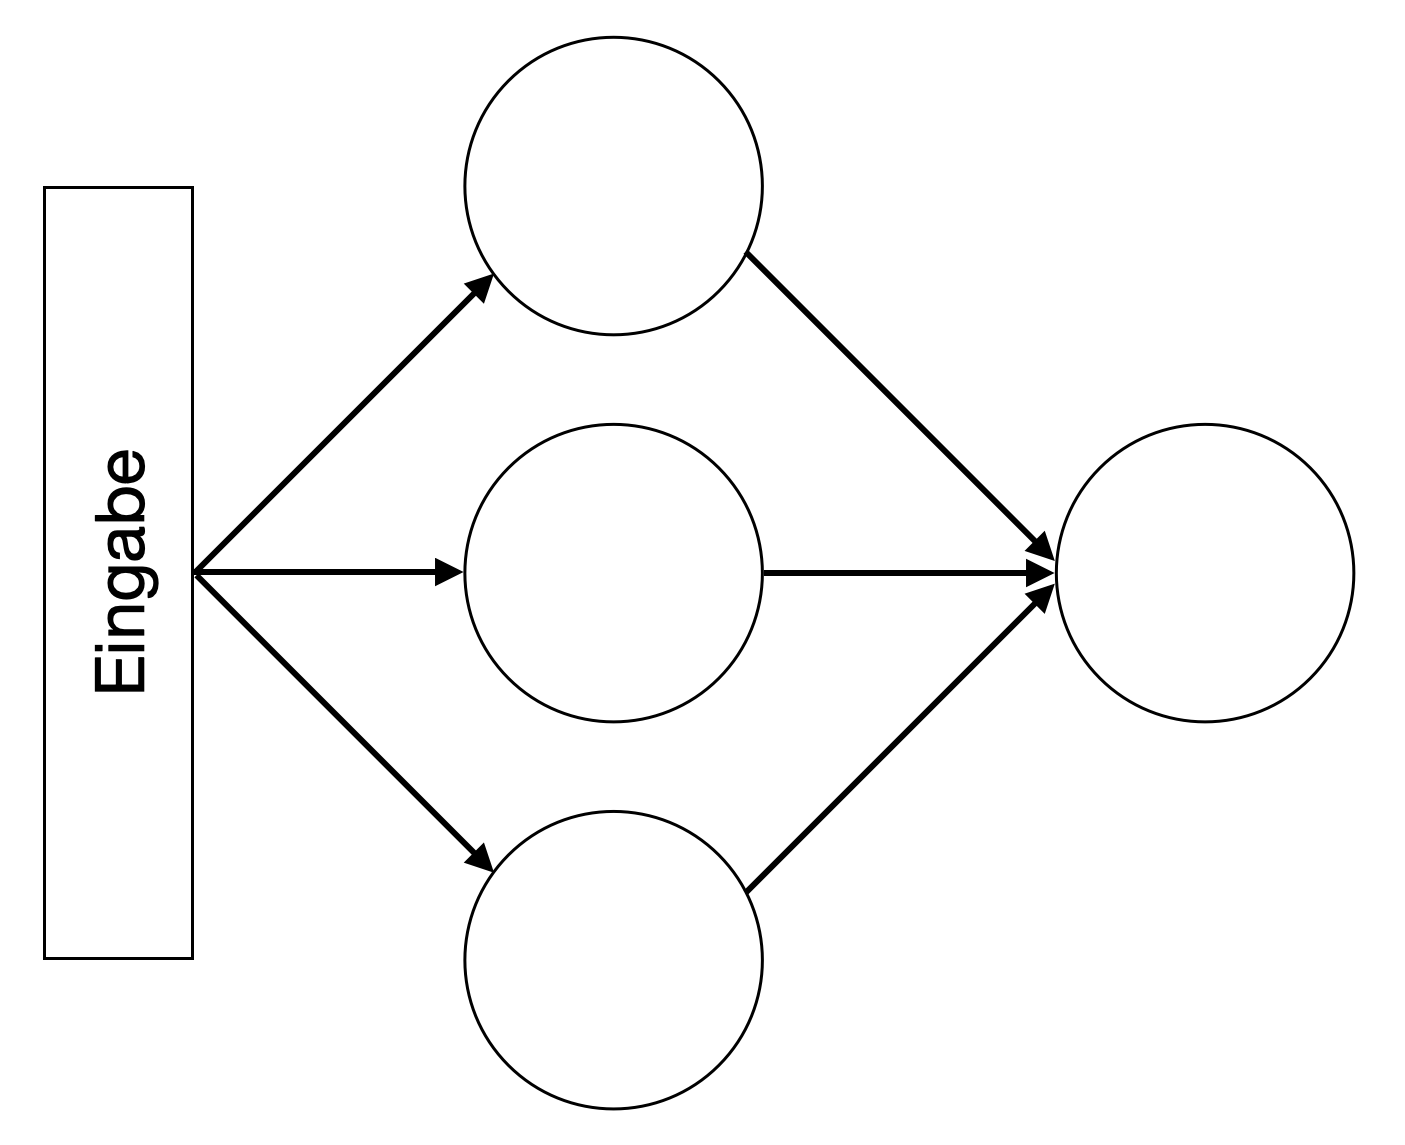
\includegraphics[width=0.75\textwidth]{bilder/singlelayernn.png}
	\caption[Ein-Schicht-NN]{Ein-Schicht-NN (Die Ausgabeschicht wird nicht mitgezählt)}
	\label{fig:singlelayernn}
\end{figure}

Logistic Regression kann mit einer einzelnen oder mehreren neuronalen Schichten imlementiert sein. Das künstliche neuronale Netz in \ref{fig:singlelayernn} besitzt eine einzelne aus drei Einheiten bestehende Schicht. Eine Einheit besteht zunächst aus einer differenzierbaren Funktion. Oft ist das eine Multiplikation der Eingaben $X$ mit einer Anzahl lernbaren Parametern $W$ und eine anschließende Addition mit Bias-Werten $b$. Die Ausgabe einer Schicht wird oft mit $\hat{y}$ bezeichnet:
\begin{align}
\hat{y} = WX+b
\end{align}

Dieser folgt eine Aktivierungsfunktion, die dem errechneten Wert einen anderen Wert zuordnet, der entweder nahe $0$ oder nahe $1$ liegt (gelegentlich nahe $-1$ oder nahe $1$). Beispiele für Aktivierungsfunktionen sind Sigmoid:
\begin{align}
sig(t) = \frac{1}{1+e^{-t}}
\end{align}

und Rectified Linear Unit, kurz ReLU:
\begin{align}
f(x) = max(0, x)
\end{align}

oder auch Leaky ReLU:
\begin{align}
f(x) = max(0.01x, x)
\end{align}

In einigen künstlichen neuronalen Netzen werden zusätzlich die Eingaben für jede Schicht normalisiert, wodurch die Minimierung der Verlustfunktion (Gradient Descent) optimiert werden kann.

\section{Deep Neural Networks}
\label{sec:dnn}

Die nachfolgende Beschreibung zu Deep Neural Networks ist in dem Buch ``Deep Learning with Python'' \cite{chollet2021deep} zu finden:

Deep Learning ist ein spezifisches Gebiet des maschinellen Lernens: Ein neuer Ansatz zum Lernen von Repräsentationen von Daten, der den Schwerpunkt auf das Lernen in aufeinanderfolgenden Schichten mit zunehmend aussagekräftigen Repräsentationen legt. Das ``Deep'' in ``Deep Learning'' ist kein Hinweis auf ein durch diesen Ansatz erlangtes tieferes Verständnis, sondern steht für diese Idee von aufeinanderfolgenden Schichten von Repräsentationen.

Die Anzahl der Schichten, aus denen ein Datenmodell zusammengefasst ist, wird Tiefe (engl.: depth) des Modells genannt. Andere passende Namen für dieses Feld hätten ``layered representations learning'' oder ``hierarchical representations learning'' sein können. Modernes Deep Learning umfasst oft mehrere zehn- oder hunderttausend aufeinanderfolgendende Repräsentationsschichten, die alle automatisch durch Verrechnung von Trainingsdaten erlernt werden.

Währenddessen gehen andere Ansätze des maschinellen Lernens eher in die Richtung des ``shallow learning'', beschränken sich also auf eine oder zwei Repräsentationsschichten. Diese Schichten von Repräsentationen werden fast immer durch Modelle erlernt, die neuronale Netze genannt werden. Diese Modelle sind buchstäblich wie aufeinander gestapelte Schichten strukturiert.

Der Begriff neuronales Netz ist ein Referenz auf Neurobiologie, doch obwohl die Entwicklung einiger zentraler Deep-Learning-Konzepte teilweise durch unser Verständnis des Gehirns inspiriert war, sind Deep-Learning-Modelle keine Modelle des Gehirns. Es gibt keine Anhaltspunkte darauf, dass das Gehirn etwas vergleichbares wie die Lernmechanismen implementiert, die in modernen Deep-Learning-Modellen verwendet werden. Gelegentlich begegnen einem populärwissenschaftliche Artikel in denen proklamiert wird, dass Deep Learning wie das Gehirn funktioniert oder nach dem Vorbild eines Gehirns modelliert wurde. Das ist aber nicht der Fall. Für Neueinsteiger in das Fachgebiet wäre es verwirrend und kontraproduktiv, Deep Learning als etwas zu betrachten, das mit Neurobiologie in irgend einem Zusammenhang steht. Deep Learning ist ein mathematisches Gerüst zum Lernen von Repräsentationen von Daten.

Ein Deep-Learning-Netzwerk ist wie ein mehrstufiger Informations-Destilliations-Vorgang, bei dem Information durch aufeinanderfolgende Filter fließt und zunehmend bereinigt und für einen bestimmten Zweck nutzbar wieder herauskommt. Die Idee hinter Deep Learning ist einfach, kann aber wie Magie anmuten, wenn der simple Mechanismus ausreichend skaliert wird.
\cite{chollet2021deep}

\section{Convolutional Neural Networks}
\label{sec:cnn}
Für Bilddaten verarbeitet ein Convolutional Neural Network, kurz CNN, typischerweise Paare von Tensoren dritter Stufe, nämlich einerseits auf die Eingabedaten und andererseits auf einen sogenannten Filter oder auch Kernel. Die Eingabedaten sind in der ersten Schicht des Netzes die RGB-Pixelinformationen und in allen weiteren konvolutionalen Schichten die Ausgabe der vorherigen Schicht. Ein Filter ist eine Anzahl von trainierbaren Parametern, enthalten in einem Tensor.

Die Form der Tensoren variiert üblicherweise zwischen den verschiedenen Schichten des Netzes. In fast allen CNNs ( \cite{isola2018imagetoimage}, \cite{goodfellow2016deeplearning}, \cite{Lecun99objectrecognition}, \cite{RFB15a}) nimmt die Dimensionalität zunächst ab. Die Reduktion kann durch die Konvolution selbst entstehen oder durch Pooling-Schichten.

Beim Pooling werden aus benachbarten Matrixkoeffizienten meist das Maximum, seltener der Durchschnitt oder andere Aggregierungen gebildet. Auf diese Weise wird das neuronale Netz darauf trainiert die relevanten Informationen zu extrahieren. \cite{goodfellow2016deeplearning}

Den konvolutionalen Schichten folgt in einigen Anwendungsfällen eine voll vernetzte Schicht (engl. Fully Connected Layer, FC), in der für jede Einheit mit jeder Einheit der vorherigen Schicht eine Verbindung besteht. Besonders für die Bilderkennung wird diese Architektur gelegentlich erfolgreich eingesetzt. Die Ausgabe des neuronalen Netzes ist dann ein Vektor, beispielsweise von Wahrscheinlichkeitswerten für das Vorhandensein bestimmter Objekte und gegebenenfalls Bildkoordinaten der erkannten Objekte. Im Fall der Bildgenerierung kann die Ausgabe aber auch wieder ein Tensor mit RGB-Pixelinformationen in der Form $(H\ x\ B\ x\ 3)$ sein.

\section{Batch Normalization}
In ``Deep Learning with Python`` \cite{chollet2021deep} ist Batch Normalization wie folgt beschrieben:

Normalisierung ist eine breit gefächerte Kategorie von Methoden, die versuchen verschiedene Eingaben für Modelle des maschinellen Lernens einander ähnlicher aussehen zu lassen. Das soll dem Modell helfen zu lernen und für neue Daten zu verallgemeinern. Die verbreitetste Form von Normalisierung besteht darin die Daten an $0$ zu zentrieren und mit einer Standardabweichung von $<1$ zu versehen, indem der Mittelwert aller Werte von jedem Einzelwert subtrahiert wird und jeder Einzelwert durch die Standardabweichung geteilt wird. Dies geschieht aufgrund der Annahme, dass die Daten normalverteilt sind und stellt sicher, dass diese Verteilung zu einer einheitlichen Varianz zentriert und skaliert ist.

Datennormalisierung sollte nach jedem Transformationsschritt durch das künstliche neuronale Netz geschehen. Auch wenn die Daten, die in ein Dense Net oder Convolutional Neural Net eingegeben werden, den Mittelwert $0$ und eine Standardabweichung $< 1$ besitzen, ist ohne weiteres nicht zu erwarten, dass es sich bei den Ausgabedaten genauso verhält.

Batch Normalization ist eine Art von Schicht, die 2015 von Ioffe und Szegedy \cite{ioffe2015batchnorm} eingeführt wurde. Sie kann adaptiv die Daten normalisieren, wenn sich Mittelwert und Varianz im Laufe des Trainings verändern. Das erreicht sie, indem sie einen exponentiellen gleitenden Durchschnitt der batchweisen Mittelwerte und Varianzen der Daten während des Trainings vorhält.

Hauptsächlich hilft die Batch Normalization bei der Backpropagation und erlaubt so tiefere Netzwerke. Einige sehr tiefe Netwerke können überhaupt nur trainiert werden, wenn sie mehrere Batch-Normalization-Schichten enthalten. Batch Normalization wird zum Beispiel in vielen fortgeschrittenen ConvNet-Architekturen verwendet, die Keras zur Verfügung stellt, wie ResNet50, Inception v3 und Xception. Eine Batch-Normalisierungs-Schicht wird typischerweise nach einem convolutional oder einer Densely-Connected-Schicht verwendet.
\cite{chollet2021deep}

\section{U-Net-Architektur}
\label{sec:unet}
Die bis hierhin beschriebenen neuronalen Netze besitzen eine gradlinige Struktur, in der die Ausgabe einer Schicht nur an die nächste Schicht übergeben wird. Bei zunehmender Anzahl der Schichten verbessert sich die Performance neuronaler Netze mit diesem Aufbau zunächst, aber verschlechtert sich bei zu vielen Schichten wieder. In einem Residual Neural Network (ResNet) verhindern zusätzliche Verbindungen zwischen nicht direkt aufeinanderfolgenden Schichten diesen Performanceverlust.

Ein U-Net ist eine spezielle Form eines ResNets. Es hat eine annähernd symmetrische Struktur, in der sich die Tensoren zunächst zunehmend verformen und anschließend wieder annähernd ihre ursprüngliche Form annehmen.

U-Nets erzielen selbst mit wenigen Trainingsdaten gute Ergebnisse und benötigen dafür vergleichsweise wenig Rechenleistung \cite{he2015deep}.

\section{Generative Adversarial Networks}
\label{gan}
Ein Generative Adversarial Network (GAN) besteht zunächst aus einem Generator und einem Discriminator. Der Generator lernt während des Trainings täuschend echt aussehende Bilddaten zu generieren. Der Discriminator wird dagegen darauf trainiert, echte von generierten Bildern zu unterscheiden. Anschließend können beide Modelle ``gegeneinander antreten''. Deswegen wird es Generative \textit{Adversarial} Network genannt.

Generative Adversarial Networks basieren auf einem spieltheoretischen Szenario, in dem das Generator-Netzwerk gegen einen Kontrahenten antreten muss. Das Generator-Netzwerk produziert Proben $\boldsymbol{x}=g(\boldsymbol{z}; \boldsymbol{\theta}^{(g)})$. Sein Kontrahent, das Discriminator-Netzwerk, versucht zwischen den Proben aus den Trainingsdaten und den vom Generator erstellten Proben zu unterscheiden. Der Discriminator gibt einen Wahrscheinlichkeitswert aus, der durch $d(\boldsymbol{x}; \boldsymbol{\theta}^{(d)})$ gegeben ist und der die Wahrscheinlichkeit angibt, dass $\boldsymbol{x}$ ein echtes Trainingsexemplar ist und keine Täuschung, die durch das Modell erstellt wurde. \cite{goodfellow2016deeplearning}

GANs unterscheiden sich von anderen Modellen durch ihren Aufbau und in Bezug auf das Trainingsziel. Künstliche neuronale Netze ermitteln häufig einen skalaren Wert wie beispielsweise einen Wahrscheinlichkeitswert und minimieren zu diesem Zweck eine Verlustfunktion. In einem GAN sind zwei CNNs im Einsatz. Das erste, der Generator, erstellt Tensoren n-ter Klasse. In diesem Beispiel sind das RGB-Bildinformationen. Das zweite CNN wird Discriminator genannt und bekommt als Eingabe die Ausgabe des ersten CNNs. Der Discriminator wird darauf trainiert, generierte Bilder von Bildern aus dem Trainingsset zu unterscheiden. Er minimiert also eine Verlustfunktion. Der Generator wird darauf trainiert, diese Verlustfunktion zu maximieren. Dieser Vorgang heißt auch Min-Max-Spiel. \cite{goodfellow2014generative}

\section{Conditional Generative Adversarial Nets}
\label{cgan}

Mehdi Mirza beschreibt in seinem Artikel ``Conditional Generative Adversarial Nets'' \cite{mirza2014conditional} eine Klasse von künstlichen neuronalen Netzen, die gegenüber Generative Adversarial Networks noch weitere Vorteile bieten:

Eine Erweiterung des GANs ist das Conditional Generative Adversarial Net (cGAN). In cGANs erhält der Generator zusätzliche Eingabedaten ($y$, ``Ground Truth''), die Hinweise für die Generierung enthalten. Der Discriminator erhält diese zusätzlichen Daten ebenfalls, um die Erkennung während des Trainings zu optimieren.

Dieses Modell kann Ziffern des MNIST-Datasets anhand von Klassenlabels generieren. Es kann auch verwendet werden, um multimodales Bild-Tagging durchzuführen. Dabei kann ein Bild beispielsweise nicht nur durch ein darauf erkennbares Objekt, sondern auch durch Aufzählung mehrerer unterschiedlicher Objekte und noch durch weitere Beschreibungen, wie erkennbare Jahreszeiten, Vorgänge oder Emotionen beschrieben werden.

In einem generativen Modell ohne Konditionen ist keine Steuerung der Art und Weise (Modalitäten) möglich, in der die Ergebnisse generiert werden. Dagegen ist es in einem cGAN möglich, die Generierung zu lenken. Diese Lenkung könnte aufgrund von Klassenlabels oder auch verschiedensten anderen Modalitäten erfolgen.

Um die Verteilung $p_g$ eines Generators über die Daten $x$ zu lernen, implementiert der Generator $G(z;\theta_g)$ eine Mapping-Funktion von anfänglichem Rauschen $p_z(z)$ zum Ergebnisraum. Der Discriminator $D(x;\theta_d)$ gibt einen einzelnen skalaren Wahrscheinlichkeitswert dafür, dass $x$ aus den Trainingsdaten statt aus $p_g$ stammt, aus.

$G$ und $D$ werden simultan trainiert. Die Parameter für G werden angepasst, um $\log(-D(G(z)))$ zu minimieren und die Parameter für $D$ werden angepasst, um $\log D(x)$ zu minimieren, so als würden beide ein Zweispieler-Min-Max-Spiel mit der Wertfunktion durchführen:
\begin{align}
\min_{G}\max_{D} V(D,G) = \mathbb{E}_{x\sim p_{data}(x)}[\log{D(x)}]+\mathbb{E}_{z\sim p_z(z)}[\log(1-D(G(z)))].
\end{align}

Im Generator werden das anfängliche Rauschen $p_z(z)$ und $y$ kombiniert in verbundenen Hidden Layers repräsentiert. Das gegnerische Trainingsframework erlaubt eine flexible Zusammensetzung dieser Repräsentation.

Im Discriminator werden paarweise $x$ und $y$ sowie $x$ und $G(z|y)$ als Eingaben verwendet. Die Funktion, die das Ziel dieses Zweispieler-Min-Max-Spiels beschreibt ist dann:
\begin{align}
\min_{G}\max_{D} V(D,G) = \mathbb{E}_{x\sim p_{data}(x)}[\log{D(x|y)}]+\mathbb{E}_{z\sim p_z(z)}[\log(1-D(G(z|y)))].
\end{align}
\cite{mirza2014conditional}

\chapter{Implementierung}
\label{ch:imple}

\section{Ubuntu Linux}
\label{sec:ubuntu}
Ubuntu ist eine der bekanntesten Linux-Distributionen. Es ist kostenlos und in verschiedenen Editionen für unterschiedliche Zwecke erhältich. Es kann beispielsweise für Server oder für Desktop-Computer verwendet werden.

Die Wahl des Betriebssystems fiel für dieses Projekt auf Ubuntu, weil die Integration mit der NVIDIA-Grafikkartenerweiterung CUDA mit Abstand am besten dokumentiert ist. Es gibt sowohl für Ubuntu als auch für CUDA eine lebendige Community. Dadurch besteht bei eventuell auftretenden Schwierigkeiten stets die Möglichkeit, auf die Erfahrungen anderer Nutzer zurückzugreifen.

Die Installation des Betriebssystems ist vergleichsweise einfach. Ein Volume-Image im ISO-Dateiformat (ISO 9660) kann vom Ubuntu-eigenen Server heruntergeladen und anschließend entweder auf eine CD oder DVD gebrannt oder auf einen bootfähigen USB-Stick kopiert werden.

Der Software-Assistent des Installationsprogramms hat eine leicht zu bedienende grafische Benutzeroberfläche. Es können alle wichtigen Einstellungen wie Eingabe- und Ausgabesprache, Uhrzeit und Sicherheitseinstellungen vorgenommen werden.

Es ist auch möglich, Ubuntu unter Windows innerhalb der WSL (Windows Subsystem for Linux) zu installieren. Auch dort besteht die Möglichkeit, die Hardwareunterstützung zu nutzen. Ubuntu unter WSL ist dann in der Lage, mittels CUDA die GPU für das Training neuronaler Netze zu verwenden.

Für diese Arbeit wurde Ubuntu als Hauptbetriebssystem genutzt. Die Schritte zur Einrichtung einer Entwicklungsumgebung für maschinelles Lernen sind auf ubuntu.com\footnote{https://ubuntu.com/tutorials/enabling-gpu-acceleration-on-ubuntu-on-wsl2-with-the-nvidia-cuda-platform/} beschrieben.

\section{Python}
\label{sec:python}
Die Programmiersprache Python ist eine beliebte Wahl für Software-Projekte im Bereich des maschinellen Lernens. Ein wichtiger Grund dafür sind die verschiedenen verfügbaren Bilbiotheken, die zum Beispiel Bausteine für künstliche neuronale Netze und sogar häufig Algorithmen bereitstellen. Zwei der berühmtesten Bibliotheken dieser Art sind TensorFlow und Keras. In dem O'Reilly-Buch ``Python'' von Mark Lutz \cite{lutz2013python} wird Python wie folgt beschrieben:

Python ist eine beliebte, quelloffene Programmiersprache sowohl für eigenständige Programme als auch für Anwendungs-Skripte in vielen verschiedenen Bereichen. Es ist kostenlos, portabel sowie relativ einfach und wird  mit bemerkenswertem Enthusiasmus verwendet.

Version 3.0 war die erste in einer Reihe der aufstrebenden und nicht abwärtskompatiblen Abwandelung der Sprache die allgemein als 3.X bezeichnet wird. Version 2.6 behielt die Abwärtskompatibilität zu einer zahllosen Menge bestehenden Python-Quelltextes bei und war die letzte der gemeinhin als 2.X bekannten Reihe.

Für viele hebt sich Python durch seinen Fokus auf Lesbarkeit, Stimmigkeit und Softwarequalität insgesamt aus anderen Tools der Skripting-Welt hervor. Python-Quelltext ist gemacht, um lesbar und dadurch wiederverwendbar und wartbar zu sein -- noch viel mehr als traditionelle Skriptsprachen. Die Gleichförmigkeit von Python-Quelltext macht ihn leicht verständlich, selbst wenn man ihn nicht selbst gegschrieben hat. Zusätzlich unterstützt Python fortgeschrittene Mechanismen für wiederverwendbare Software, wie objektorienterte und funktionale Programmierung.

Python erhöht die Entwicklerprodutkivität um einiges mehr als kompilierte oder statisch typisierte Sprachen wie C, C++ und Java. Die Größe von Pythoncode ist typischerweise ein Drittel bis ein Fünftel von der equivalenten C++- oder Java-Quelltexts. Das heißt es gibt weniger zu tippen, weniger zu debuggen und schließlich weniger zu warten. Python-Programme sind auch unmittelbar ausführbar, ohne die langwierigen Kompilier- und Linkschritte, die für manche anderen Tools erforderlich sind, und erhöht die Programmierergeschwindigkeit somit noch weiter.

Die meisten Python-Programme laufen unverändert auf allen wichtigen Computerplattformen. Um Pythoncode zwischen Lunux und Windows zu portieren, ist es zum Beispiel gewöhnlich nur erforderlich den Skriptcode von einer Maschine zur anderen zu kopieren. Überdies bietet Python multiple Optionen für die Erstellung portabler grafischer Benutzerschnittstellen, Datenbankanwendungen, webbasiserter Systeme und anderem. Selbst Betriebssystemschnittstellen, einschließlich Programmausführungen und Verzeichnisverarbeitung sind so portable wie irgend möglich.

Python enthält eine große Sammlung vorgefertigter und portabler Funktionalitäten, bekannt als die Standardbibliothek. Diese Bibliothek unterstützt eine Reihe von Programmieraufgaben auf Anwendungsebene, von Musterkennung in Texten bis Netzwerkprogrammierung. Außerdem kann Python sowohl mit selbstentwickelten Bilbiotheken als auch einer unüberschaubaren Kollektion von Unterstützungssoftware dritter erweitert werden. Pythons Drittanbieter-Bereich bietet Tools zur Webseitenerstellung, numerische Programmierung, Zugriff auf serielle Ports, Spieleentwicklung und vieles mehr. Die Erweiterung NumPy wird zum Beispiel als kostenloses und mächtigeres Equivalent zum numerischen Programmiersystem Matlab bezeichnet.

Pythonskripte können leicht mit anderen Teilen einer Anwendung kommunizieren, indem sie eine Vielzahl integrierter Mechanismen nutzen. Solche Integrationen erlauben es, Python als Produktanpassungs- und Produkterweiterungstool zu verwenden. Pythoncode kann heute C- und C++-Bibliotheken aufrufen, von C- und C++-Programmen aufgerufen werden, in Java- und .NET-Komponenten integriert werden, mittels Frameworks wie COM und Silverlight kommunizieren, sich mit Geräten via serieller Schnittstelle verbinden und über Netzwerke mit Schnittstellen wie SOAP, XML-RPC und CORBA interagieren. Es ist kein alleinstehendes Tool. \cite{lutz2013python}

\section{CUDA}
\label{sec:cuda}
Cuda ist eine NVIDIA-proprietäre Hardware- und Software-Architektur. Auch zu CUDA existiert ein Buch. Es heißt ``CUDA by Example: An Introduction to General-Purpose GPU Programming'' \cite{sanders2010cuda} und enthält die folgende Beschreibung:

Die CUDA-Architektur ist das Schema, nach dem NVIDIA-Grafikkarten gebaut wurden, die sowohl traditionelle Grafik-Rendering-Aufgaben als auch allgemeine Aufgaben durchführen können. Zum Programmieren der CUDA GPUs wird die Sprache CUDA C verwendet. CUDA C ist im Wesentlichen die Programmiersprache C mit einer Handvoll Erweiterungen, welche die Programmierung hoch parallelisierter Maschinen wie NVIDIA GPUs ermöglichen.

Anders als frühere GPU-Generationen, die Rechenressourcen in Vertex- und Pixelshader aufteilten, enthält die CUDA-Architektur eine einheitliche Shader-Pipeline, welche die Zuordnung allgemeiner Berechnungen zu jeder arithmetisch-logischen Einheit (ALU) auf dem Chip durch ein Programm erlaubt. Diese ALUs wurden mit einem Befehlssatz entworfen, der für allgemeine Berechnungen statt für spezielle Grafikberechnungen zugeschnitten ist. Weiterhin wurde den Execution Units auf der GPU freier Lese- und Schreibzugriff auf den Speicher sowie Zugriff auf einen softwaregesteuerten Cache, genannt Shared Memory, gegeben.

Zusätzlich zu der Sprache für das Schreiben von Code für die GPU stellt NVIDIA einen spezialisierten Hardwaretreiber zur Verfügung, der die hohe Rechenleistung der CUDA-Architektur ausschöpft. Kenntnis der OpenGL- oder DirectX-Programmierschnittstellen ist nicht länger erforderlich. \cite{sanders2010cuda}

\section{Image-To-Image-Translation in Python}
\label{sec:pix2pix}
Der Image-To-Image-Translation-Algorithmus oder kurz Pix2Pix-Algorithmus verwendet ein GAN, um Bilder in Bilder zu übersetzen. Dafür kommen zwei CNNs zum Einsatz, nämlich eins für den Generator und eins für den Discriminator. \cite{isola2018imagetoimage}

Die Datei \hyperref[pix2pixpy]{main.py befindet sich im Anhang 1}. Es ist eine Beispielimplementierung zum Artikel ``Image-to-Image Translation with Conditional Adversarial Networks'' \cite{isola2018imagetoimage} und ist im Github-Repository tensorflow/docs\footnote{\href{https://github.com/tensorflow/docs/blob/master/site/en/tutorials/generative/pix2pix.ipynb}{https://github.com/tensorflow/docs/blob/master/site/en/tutorials/generative/pix2pix.ipynb}} zu finden. Für meine Experimente habe ich hauptsächlich diese Implementierung verwendet. Sie wurde für die erste Hauptversion von Tensorflow geschrieben und war zunächst mit meinem Setup nicht ausführbar. Deshalb folgen den Import-Anweisungen am Anfang des Python-Skripts weitere Imports und Konfigurationen, um die Kompatibilität herzustellen. Im Verlauf des Programmes wird dann die erste Tensorflow-Version genutzt.

Eine weitere Änderung ist das selbst erstellte Dataset, das statt der im Beispiel verwendeten Gebäudefassaden geladen wird. Es wurden auch Ausgaben entfernt, wegen derer die Ausführung des Skriptes unterbrochen wurde. Dabei wurden Bildinformationen und Beispielbilder nach dem Laden des Datasets, dem Aufteilen in Eingabebild und Ground Truth, der Erzeugung von Bildrauschen, Down- und Upsampling sowie den ersten Trainingsdurchläufen ausgegeben, die während des Trainings der Skizzen- und Renderbilder nicht betrachtet werden mussten. Außerdem wurden in der Original-Implementierung bei jedem Training Diagramme des Generators und des Discriminators erzeugt.

Die erste Funktion namens \lstinline|load| öffnet eine Datei und liest diese als JPEG-Bilddatei. Sie wird verwendet, um die Trainingsdaten zu laden. Weil die Trainingsdaten aus zwei Bildern pro Datei bestehen, nämlich jeweils einem Eingabebild und dem erwarteten Ergebnis (Ground Truth), extrahiert die Funktion zusätzlich die beiden Bilder und gibt jede in einer eigenen Variablen zurück.

Die Funktion \lstinline|resize| ist ebenfalls für die Verarbeitung zweier Bilder vorgesehen und skaliert beide auf die übergebene Breite und Höhe.

Die Funktion \lstinline|random_crop| stellt einen zufälligen Ausschnitt der zwei Eingabebilder frei. Sie wird aufgerufen, nachdem die Eingabebilder hochskaliert wurden. In der Beispielimplementierung wie auch in dieser Arbeit beträgt die Bildgröße vorher $286x286$ Pixel und $256x256$ Pixel nach dem Freistellen. Die zurückgegebenen Bilder haben dann wieder die gleichen Abmessungen wie die Eingabedaten.

In der Funktion \lstinline|normalize| werden die RGB-Werte der beiden Eingabebilder normalisiert. Dadurch sollen zu große Schritte auf dem Gradienten verhindert werden, die das Konvergieren verhindern könnten. \cite{chollet2021deep} Die RGB-Werte sind zunächst als Ganzzahlen im Bereich von 0 bis 255 gegeben und werden in Fließkommazahlen im Bereich -1 bis 1 umgerechnet.

In \lstinline|random_jitter| wird zunächst \lstinline|resize| aufgerufen, um die Eingabebilder auf 286x286 Pixel zu skalieren. Anschließend wird \lstinline|random_crop| auf die skalierten Bilder angewendet. Schließlich werden aufgrund einer Zufallszahl beide Eingabebilder mit einer Wahrscheinlichkeit von 50 Prozent gespiegelt.

Die beiden Funktionen \lstinline|load_image_train| und \lstinline|load_image_test| laden die Eingabe- und Zielbilder, skalieren diese auf 256x256 Pixel und normalisieren die Eingabedaten durch Aufrufe der Funktionen \lstinline|load|, \lstinline|resize| und \lstinline|normalize|. Nur die Funktion zum Laden der Trainingsbilder ruft für die geladenen Bilder \lstinline|random_jitter| auf.

Die Funktion \lstinline|downsample| erzeugt eine Schicht eines CNNs mit optionaler Batch Normalization und der Leaky-ReLU-Aktivierungsfunktion. Diese Schichten werden im Encoder des Generators sowie im Discriminator verwendet. Batch Normalization kommt nur in der jeweils ersten Schicht des Generators und des Discriminators nicht zum Einsatz.

In der Funktion \lstinline|upsample| entstehen die übrigen CNN-Schichten des Generators. Der Entfaltung, bei der die Faltung der Funktion \lstinline|downsample| umgekehrt wird (engl. Transposed Convolution \cite{zaccone2018tensorflow}), folgt hier immer die Batch Normalization sowie optional Dropout mit einem Wahrscheinlichkeitswert von $0.5$. Das ist in den ersten drei Schichten des Decoders im Generator der Fall und bedeutet, dass statistisch die Hälfte der Aktivierungen „fallengelassen“ werden, also nicht in das Trainingsergebnis eingehen. Als Aktivierungsfunktion kommt ReLU zum Einsatz.

In \lstinline|build_generator| werden die Schichten des Generators zusammengefügt. Im Encoder wird achtmal \lstinline|downsample| aufgerufen, bis die Dimensionen des Eingabetensors, die am Anfang der Bildgröße entsprechen (Breite und Höhe, also $256x256$ Pixel), durch die Konvolution auf $1$ reduziert sind. Die Dimension, welche die Anzahl Farbkanäle der Eingabebilder repräsentiert, erhöht sich im Encoder auf den Wert $512$. Die Werte dieser Achse werden als Features \cite{zhang2020dive} \cite{chollet2021deep} \cite{zaccone2018tensorflow} bezeichnet.

Der Decoder ruft seinerseits siebenmal \lstinline|upsample| auf und führt eine weitere Entfaltung durch, wodurch die Dimensionen des bearbeiteten Tensors wieder jeweils dieselbe Form wie in den Eingabebildern annehmen. Schließlich werden die Skip-Connections zwischen den Schichten 1 bis 8 des Encoders und des Decoders hergestellt.

In der Funktion \lstinline|generator_loss| ist die Backpropagation des Generators implementiert. Zuerst wird dafür die Kreuzentropie des Ergebnisses des Discriminators und eines gleich großen Tensors, der mit Einsen initialisiert wird, gebildet. Das Ergebnis ist das GAN-Loss. Anschließend kommt die L1 Loss Function, auch Mean Absolute Error genannt, zum Einsatz. Dieses L1-Loss wird aus dem Durchschnitt der absoluten Differenz der Ground Truth und des Generatorergebnisses berechnet. Der Gesamtverlust des Generators ist das GAN-Loss plus das Produkt aus dem Regularisierungsparameter Lambda, der konstant $100$ beträgt, und dem L1-Loss. Die Funktion \lstinline|generator_loss| gibt den Gesamtverlust, das GAN-Loss und das L1-Loss zurück.

In \lstinline|build_discriminator| wird der Discriminator aus verschiedenen neuronalen Schichten zusammengesetzt. Zwei Tensoren \lstinline|input_image| und \lstinline|target_image| mit denselben Anzahlen Achsen und denselben Dimensionen wie die Eingabebilder werden zu einem einzelnen Tensor konkateniert. Anschließend wird für diesen Tensor dreimal \lstinline|downsample| aufgerufen, bis der Tensor die Dimensionen $(32x32x256)$ hat. Es folgt ein Padding mit Nullen, eine weitere Konvolution sowie Batch Normalization und die Leaky ReLU Aktivierungsfunktion. Nach einem weiteren Null-Padding und einer weiteren Konvolution hat der Tensor die Dimensionen $(30x30x1)$.

In der Funktion \lstinline|discriminator_loss| ist die Backpropagation des Discriminators implementiert. Aus jeweils einem Tensor mit den gleichen Dimensionen wie die Eingabebilder und mit Einsen initialisiert wird die Kreuzentropie mit einem Trainingsbild und dem Ergebnis des Generators gebildet. Die jeweiligen Werte für den Verlust des Discriminators werden als Gesamtverlust zurückgegeben.

Die Funktion \lstinline|generate_images| verwendet das Model des Generators, um aus Eingabebildern eigene Bilder zu generieren. Sie erstellt anschließend eine Ausgabedatei mit einem Beispiel bestehend aus einem Eingabebild, der zugehörigen Ground Truth und dem daraus generierten Bild.

In der Funktion \lstinline|train_step| wird ein Generator mit dem übergebenen Input-Bild und dem ebenfalls übergebenen Target-Bild initialisiert. Außerdem werden zwei Discriminator initialisiert, nämlich einmal mit dem Input- und dem Target-Bild und einmal mit dem Input-Bild und dem durch den Generator erstellten Bild.

Die Initialisierung des Generators und der Discriminator anhand der vorliegenden Bilder werden durch das Framework aufgezeichnet. Dadurch ist es anschließend möglich, die Gradienten mittels der in \lstinline|generator_loss| und \lstinline|discriminator_loss| berechneten Fehler des Generators und des Discriminators zu berechnen, um diese Werte an die jeweiligen Optimizer zu übergeben.

Schließlich wird in \lstinline|train_step| eine maschinenlesbare Zusammenfassung des aktuellen Trainingsschrittes erstellt. In TensorBoard kann diese Zusammenfassung eingelesen werden, um den aktuellen Trainingsdurchlauf und Trainingserfolg zu beobachten und abgeschlossene Trainingsdurchläufe zu vergleichen.

\begin{figure}[h]
	\centering
	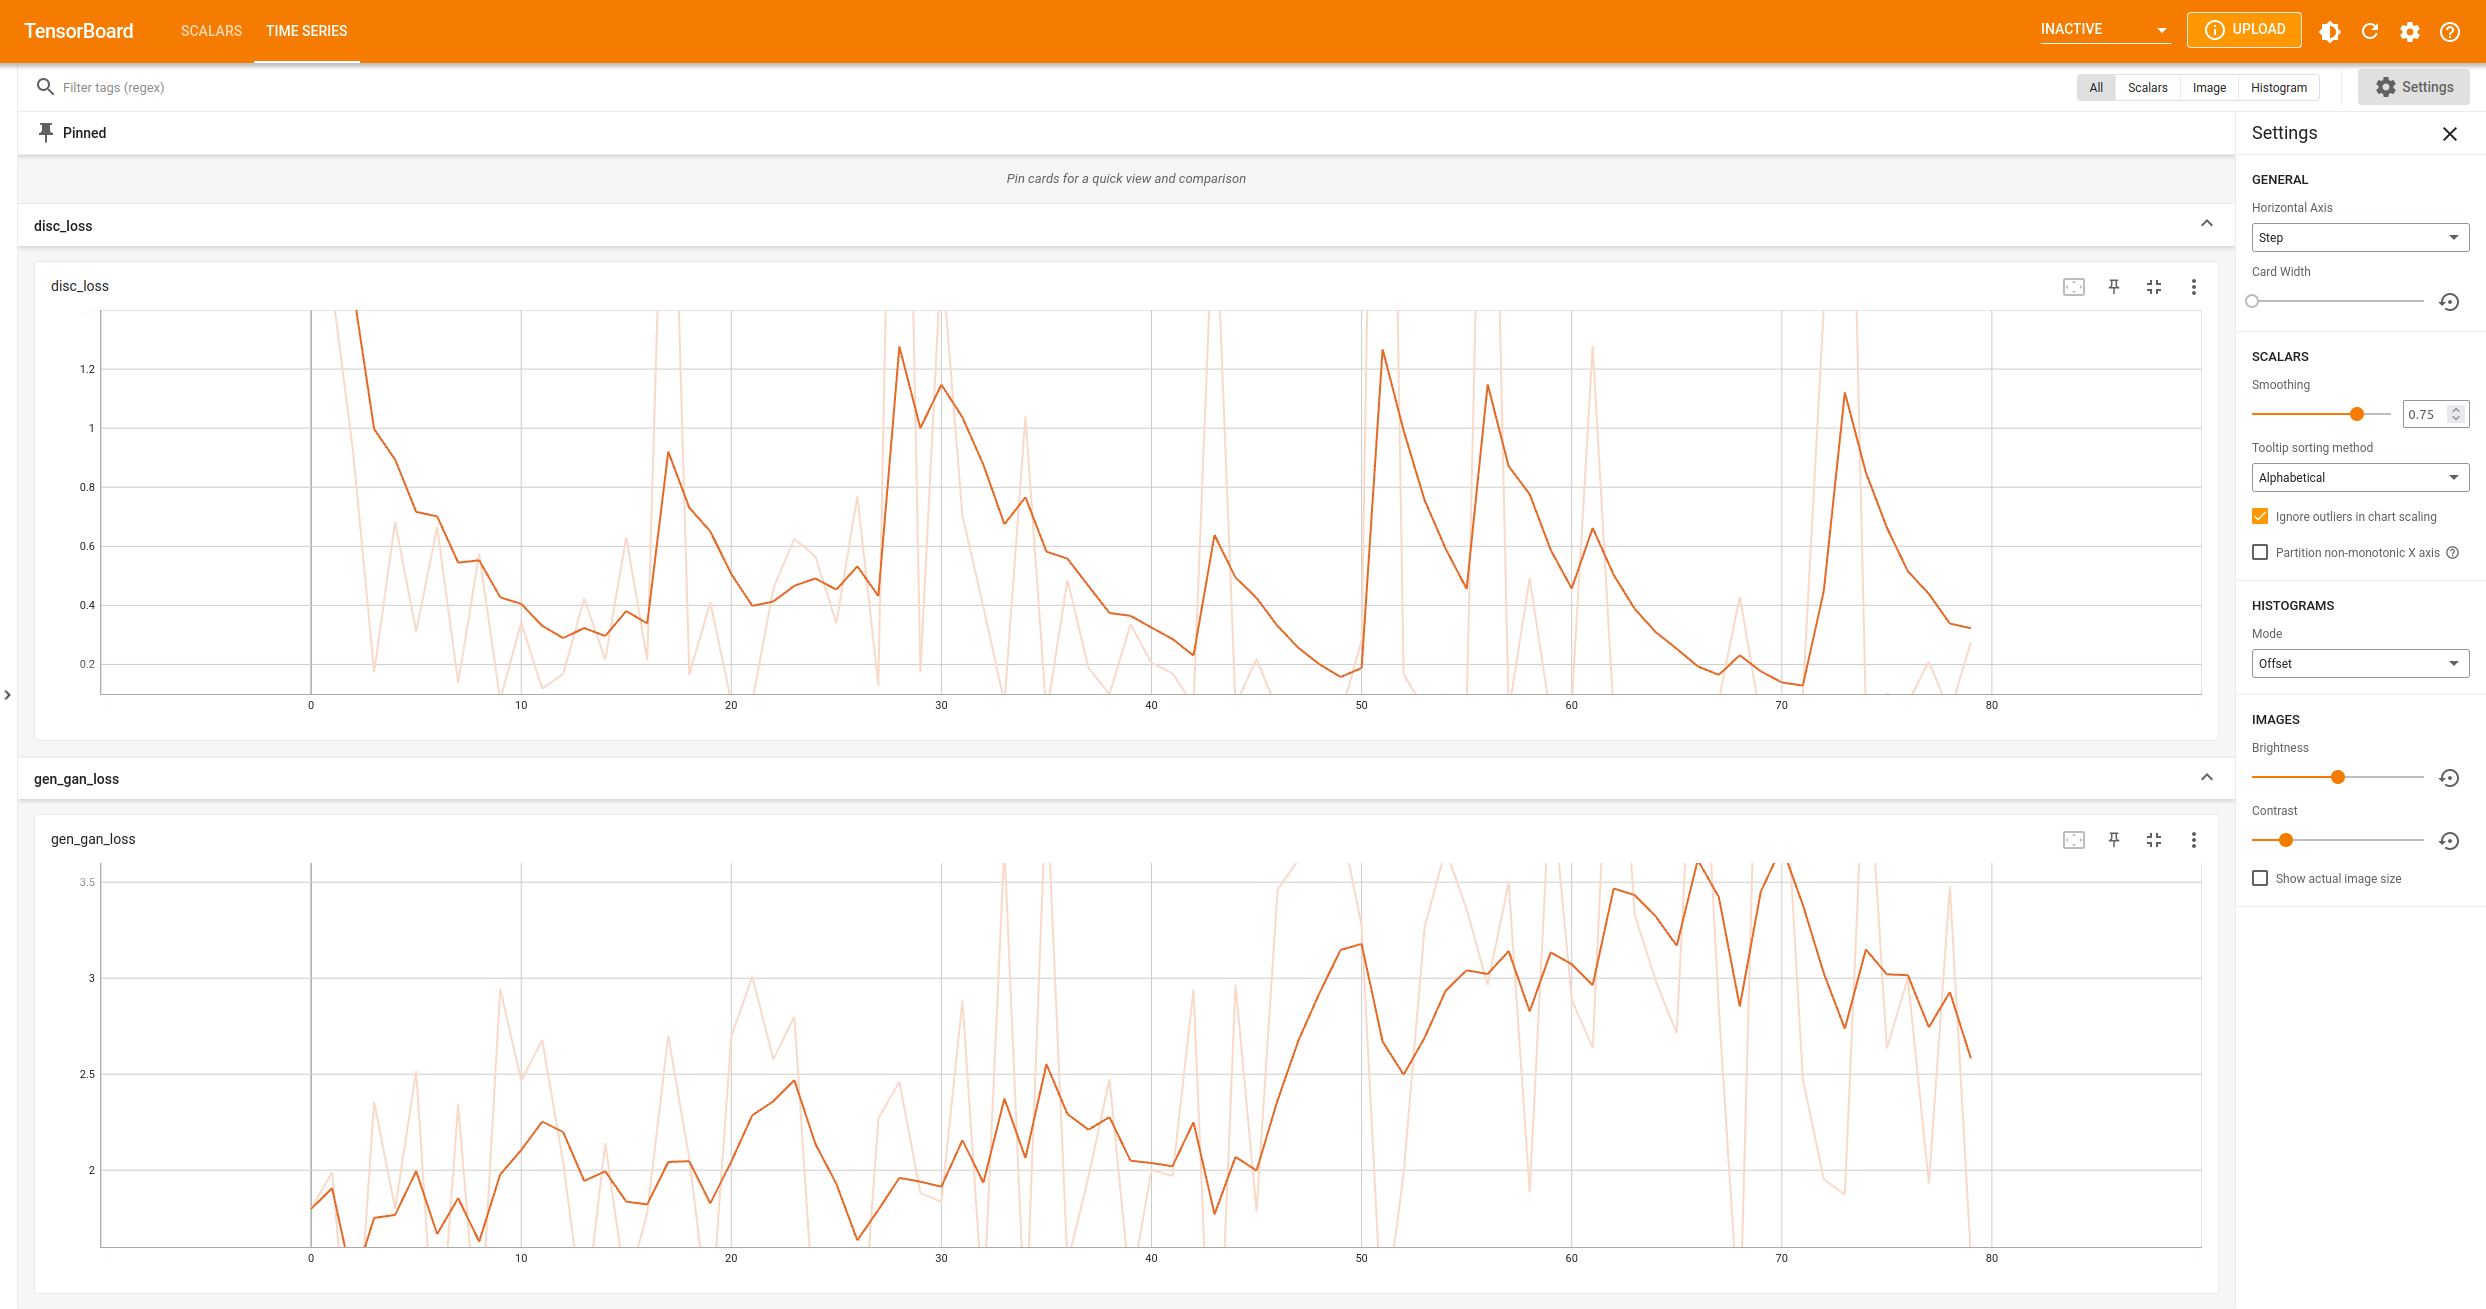
\includegraphics[width=1.0\textwidth]{bilder/tensorboard.png}
	\caption[TensorBoard]{Im TensorBoard können die Fehlerraten des aktuellen Trainingsdurchlaufs abgelesen oder frühere Trainingsdurchläufe miteinander verglichen werden.}
	\label{fig:tensorboard}
\end{figure}

In der Funktion \lstinline|fit| wird zuerst ein Bild des Testsets geladen. Das Beispielbild wird verwendet, um durch Aufrufen von \lstinline|generate_images| den aktuellen Trainingserfolg in Form einer Bilddatei im Ausgabeverzeichnis zu speichern. Dieser Vorgang erfolgt nach je 1000 Trainingsschritten.

Über die Trainingsbilder wird wiederholt iteriert und für jedes Trainingsbild \lstinline|train_step| aufgerufen.

Nach je 5000 Trainingsschritten speichert \lstinline|fit| außerdem einen Checkpoint. Dadurch kann einerseits das Training unterbrochen und zu einem späteren Zeitpunkt fortgesetzt werden. Andererseits wird das Modell auf diese Weise persistiert, und es ist später möglich, das künstliche neuronale Netz für seinen eigentlichen Einsatzzweck zu nutzen, ohne es erneut zu trainieren.

Im Ausführungsstrang wird zunächst eine Option des GPU-Speichermanagements gewählt, um die Größe des reservierten Speichers dynamisch anwachsen zu lassen \cite{zaccone2018tensorflow}. Zu Beginn der Experimente hat sich diese Einstellung in Bezug auf die Performance als vorteilhaft herausgestellt.

Es werden auch einige Parameter wie die Bildgröße und die Größe des Trainingssets und Hyperparameter wie die Batchgröße gesetzt. Das Trainings- und das Testset werden eingelesen, der Generator und die Discriminator erstellt und der Adam-Optimizer initialisiert. Nachdem anschließend das Schreiben der Checkpoints und der Zusammenfassung vorbereitet wurde, erfolgt das Training durch Aufruf von \lstinline|fit|. Im letzten Schritt wird das Modell mit 5 Beispielbildern aus dem Testset aufgerufen.

\chapter{Experimente und Resultate}
\label{ch:conduct}

\section{Vorbereitung der vorhandenen Eingabedaten}
\label{sec:preparation}
Die Trainingsdaten liegen für das ``Quick, Draw!''-Dataset im NDJSON-Format und als Blender-Dateien beziehungsweise
Wavefront OBJ-Dateien vor. Die effizienteste Möglichkeit, die Skizzen und 3D-Modelle für die Verarbeitung in einem CNN vorzubereiten, ist das Rendern und  Speichern als Bilddateien. Als Dateiformat kommen JPEG oder PNG infrage. Beide Formate können leicht als Trainingsset mit Tensorflow geladen werden.

Das ``Quick, Draw!''-Dataset steht unter der Creative-Commons-Lizenz CC BY 4.0. Eine Zusammenfassung der Lizenz ist auf creativecommons.org\footnote{\href{https://creativecommons.org/licenses/by/4.0/}{https://creativecommons.org/licenses/by/4.0/}} nachzulesen. Der Urheber ist Google, Inc. und das Material kann dem Github-Repository googlecreativelab/quickdraw-dataset\footnote{\href{https://github.com/googlecreativelab/quickdraw-dataset}{https://github.com/googlecreativelab/quickdraw-dataset}} entnommen werden. An dem Material in dem Dataset wurden durch mich keine Änderungen durchgeführt. Die Lizenz erfordert, dass diese Informationen genannt werden, was somit geschehen ist.

NDJSON steht für Newline Delimited JavaScript Object Notation. Die Spezifikation ist im Github-Repository ndjson/ndjson-spec\footnote{{https://github.com/ndjson/ndjson-spec}{https://github.com/ndjson/ndjson-spec}} zu finden. In einer solchen Datei sind also zeilenweise JSON-Objekte gespeichert. Für jede Zeichnung sind Angaben zu Motiv, Ort und Zeit enthalten. Außerdem ist angegeben, ob die künstliche Intelligenz des Minispiels das Motiv in der Zeichnung korrekt klassifiziert, also erkannt hat. Jede Zeichnung hat weiterhin eine eindeutige ID.

Der relevanteste Teil ist die ``Drawings''-Eigenschaft der JSON-Objekte, ein mehrdimensionales Array mit Bildkoordinaten. Es enthält mindestens X-Koordinaten und Y-Koordinaten in jeweils einem Array im ``Drawings''-Array. Indem Linien zwischen den Bildkoordinaten in der Reihenfolge der Arrayelemente in ein Bild gezeichnet und in einer Bilddatei gespeichert werden, können die Zeichnungen in beliebigen Bilddateiformaten gespeichert werden. Für diese Arbeit wurde die Konvertierung ebenfalls in Python implementiert.

Die Implementierung im \hyperref[ndjsonpy]{Skript im Anhang 2} beginnt mit den erforderlichen Importen, unter anderem um JSON zu dekodieren und Dateien im JPEG-Format erstellen zu können. Anschließend wird die Anzahl der zu konvertierenden Dateien festgelegt und die NDJSON-Datei als Tensorflow-Dataset vorbereitet.

In einer Schleife wird nun über die Zeilen der NDJSON-Datei iteriert. Zuerst wird der Fortschritt des Skripts auf der Konsole ausgegeben. Die nächste Zeile des Datasets wird in ein Python-Objekt dekodiert, und die ``Drawing''-Eigenschaft, in der die gezogenen Linien enthalten sind, in einer Variablen abgelegt.

Als nächstes wird die Bilddatei vorbereitet. Die Zeichnung soll als schwarze Linie auf weißem Hintergrund in einem $256x256$ Pixel großen RGB-Bild gespeichert werden. In der darauffolgenden Zeile wird ein PIL-Objekt erstellt, das Zeichenfunktionen zur Verfügung stellt.

Da eine Zeichnung fast nie die gesamte verfügbare Breite und Höhe der in dem Minigame verfügbaren Zeichenfläche auch nutzt, würde das Ergebnis ohne eine entsprechende Normalisierung der Koordinaten an der linken und der oberen Grenze des Ausgabebildes anliegen und an der rechten und unteren Seite des Bildes ein freier Rand entstehen. Deshalb werden in dem Abschnitt unter dem Kommentar \lstinline{# normalise coords to center the drawing} die Minimal- und Maximalwerte auf jeder Achse ermittelt und daraus ein Offset für die Koordinaten berechnet, um die Zeichnung im Ausgabebild zu zentrieren.

Über die Koordinaten iterierend wird die Handzeichnung dann in das RGB-Bild gezeichnet. Anschließend wird das Bild als JPEG-Datei unter einem eindeutigen Namen gespeichert.

Das Skript endet, nachdem alle Zeilen der NDJSON-Eingabedatei verarbeitet oder 5000 Bilddateien erstellt wurden.

Bei der Verarbeitung in einem Convolutional Neural Network spielt die Bildgröße
in Bezug auf die Verarbeitungszeit eine wichtige Rolle. Bildformate der Größe 256x256 oder kleiner sind üblich und gut geeignet. Für ein GAN ist es zwar nicht erforderlich, aber sinnvoll, für Ein- und Ausgabedaten dieselben Dimensionen festzulegen. Bei der Bildgenerierung aus Skizzen unterscheiden sich Ein- und Ausgabdedaten natürlich in der Farbtiefe. Während die Skizzen Graustufenbilder sind, besitzen die generierten Bilder drei Farbkanäle (RGB).

Sowohl während der Entwicklung als auch zur Laufzeit kann es vorteilhaft sein, Farbwerte statt auf der oft verwendeten Skala von $0$ bis $255$ als Fließkommazahlen im Bereich $0,0$ bis $1,0$ darzustellen. Auch für die Ausgaben der einzelnen Schichten eines künstlichen neuronalen Netzes kann diese Normalisierung durchgeführt werden.

Ein ebenso wichtiger wie aufwendiger Vorgang ist die Klassifizierung der Trainingsdaten, also die Zuweisung von Eingaben zu den erlernbaren Ergebnissen. Aufgrund der selbst erstellten Ausgabebilder existieren für diesen Zweck keine vorgefertigten Datasets. Die Sortierung und Zuweisung erfolgt deshalb manuell.
\pagebreak

\section{Erstellung eigener Eingabedaten}
\label{sec:inputdata}

Die Vorteile, die selbst erstellte Eingabedaten bieten, rechtfertigen in dieser Arbeit das Erstellen vieler eigener Eingabebilder. Dafür ist es nicht erforderlich, jedes Bild einzeln von Hand zu erzeugen. Blender verfügt über eine Python-Schnittstelle. Mit ihr ist es möglich, etwa die Ausrichtung eines dreidimensionalen Objekts automatisiert mehrmals zu ändern und jeweils ein Bild zu erstellen, sodass aus einem einzigen Modell mehrere Eingabebilder entstehen. Bei einigen Modellen wie zum Beispiel Tischen konnte sogar die Form aus zufälligen Werten für Höhe, Breite und Tiefe generiert werden.

\begin{figure}[h]
	\centering
  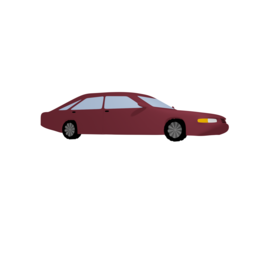
\includegraphics[width=0.325\textwidth]{bilder/limo1_m.png}
  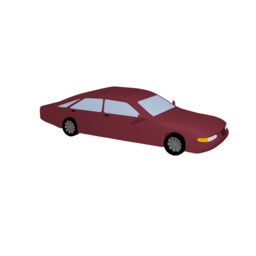
\includegraphics[width=0.325\textwidth]{bilder/limo2_m.png}
  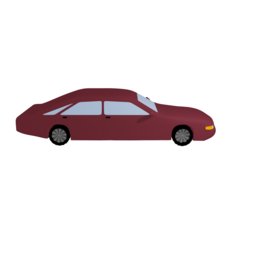
\includegraphics[width=0.325\textwidth]{bilder/limo3_m.png}

	\caption[Verschiedene Perspektiven]{3D-Modelle von Fahrzeugen können unterschiedlich in der Szene ausgerichtet werden. Dadurch entstehen verschiedene, aber homogene Eingabebilder.}
	\label{fig:limo}
\end{figure}


\begin{figure}[h]
	\centering
	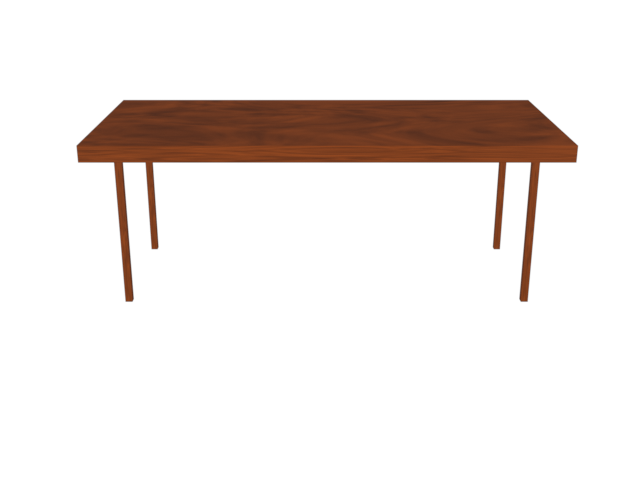
\includegraphics[width=0.325\textwidth]{bilder/random_table1_render4.png}
	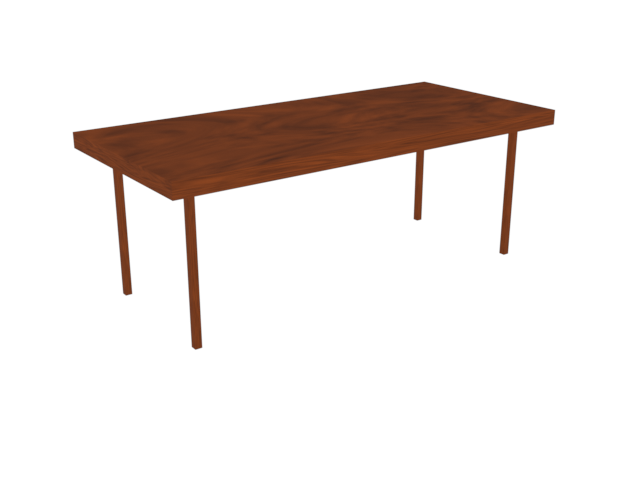
\includegraphics[width=0.325\textwidth]{bilder/random_table1_render0.png}
	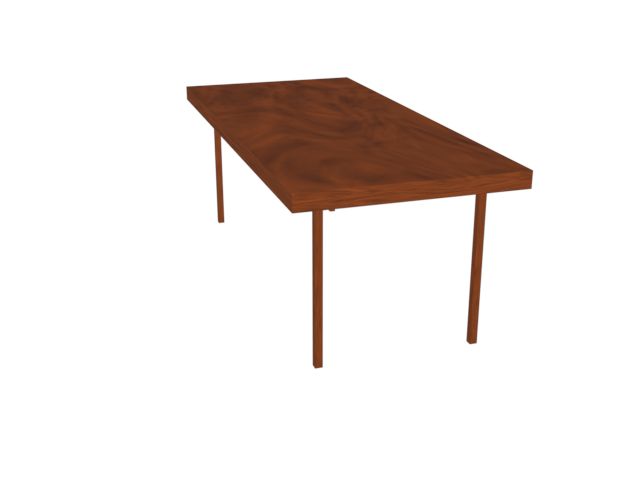
\includegraphics[width=0.325\textwidth]{bilder/random_table1_render2.png}

	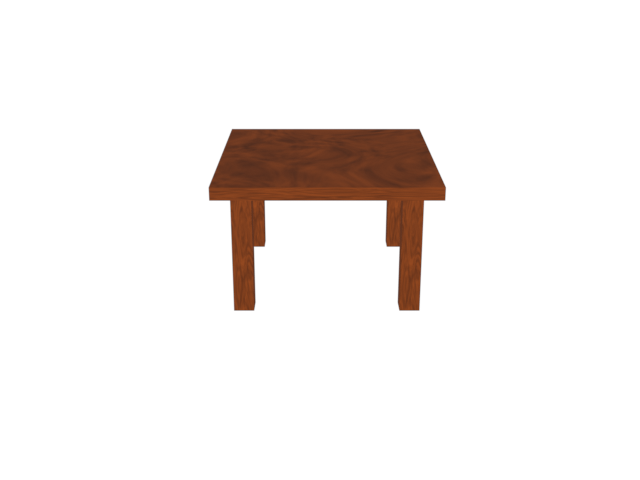
\includegraphics[width=0.325\textwidth]{bilder/random_table11_render4.png}
	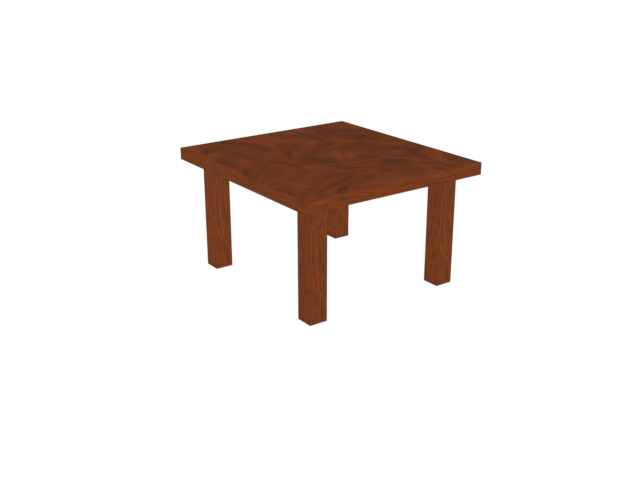
\includegraphics[width=0.325\textwidth]{bilder/random_table11_render0.png}
	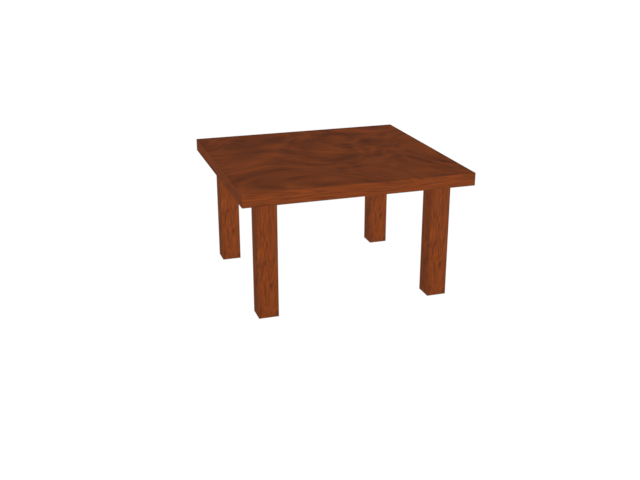
\includegraphics[width=0.325\textwidth]{bilder/random_table11_render2.png}

	\caption[Generierte Tische]{Tische können fast vollkommen automatisiert erstellt werden. Für Höhe, Breite und Tiefe der Tischbeine und Tischplatte wurden jeweils zufällige Werte innerhalb bestimmter sinnvoller Bereiche ermittelt. Dadurch konnte mit verhältnismäßig geringem Aufwand eine große Menge an Eingabebildern produziert werden.}
	\label{fig:tables}
\end{figure}

3D-Modellierungsprogramme haben prinzipiell ungewohnte Benutzeroberflächen. Das Navigieren in einer dreidimensionalen Szene erfordert Eingaben, die mittels Maus und Tastatur nicht gleichzeitig intuitiv und effizient ausgeführt werden können.

Für das Modellieren ist aber exaktes Arbeiten nötig. Ein 3D-Modellierungsprogramm muss deshalb in der Lage sein, präzise Änderungen im dreidimensionalen Raum nach den Eingaben des Benutzers durchzuführen. Blender besitzt dafür vielfältigste Funktionen. Insbesondere gibt es neben der freien Navigation im Raum verschiedene vordefinierte Perspektiven wie zum Beispiel Draufsicht und Seitenansicht. Es gibt Orientierungslinien in der Szene, an denen ein geometrisches Objekt ausgerichtet werden kann und auch sollte, um korrekt modellieren zu können.

\begin{figure}[h]
	\centering
	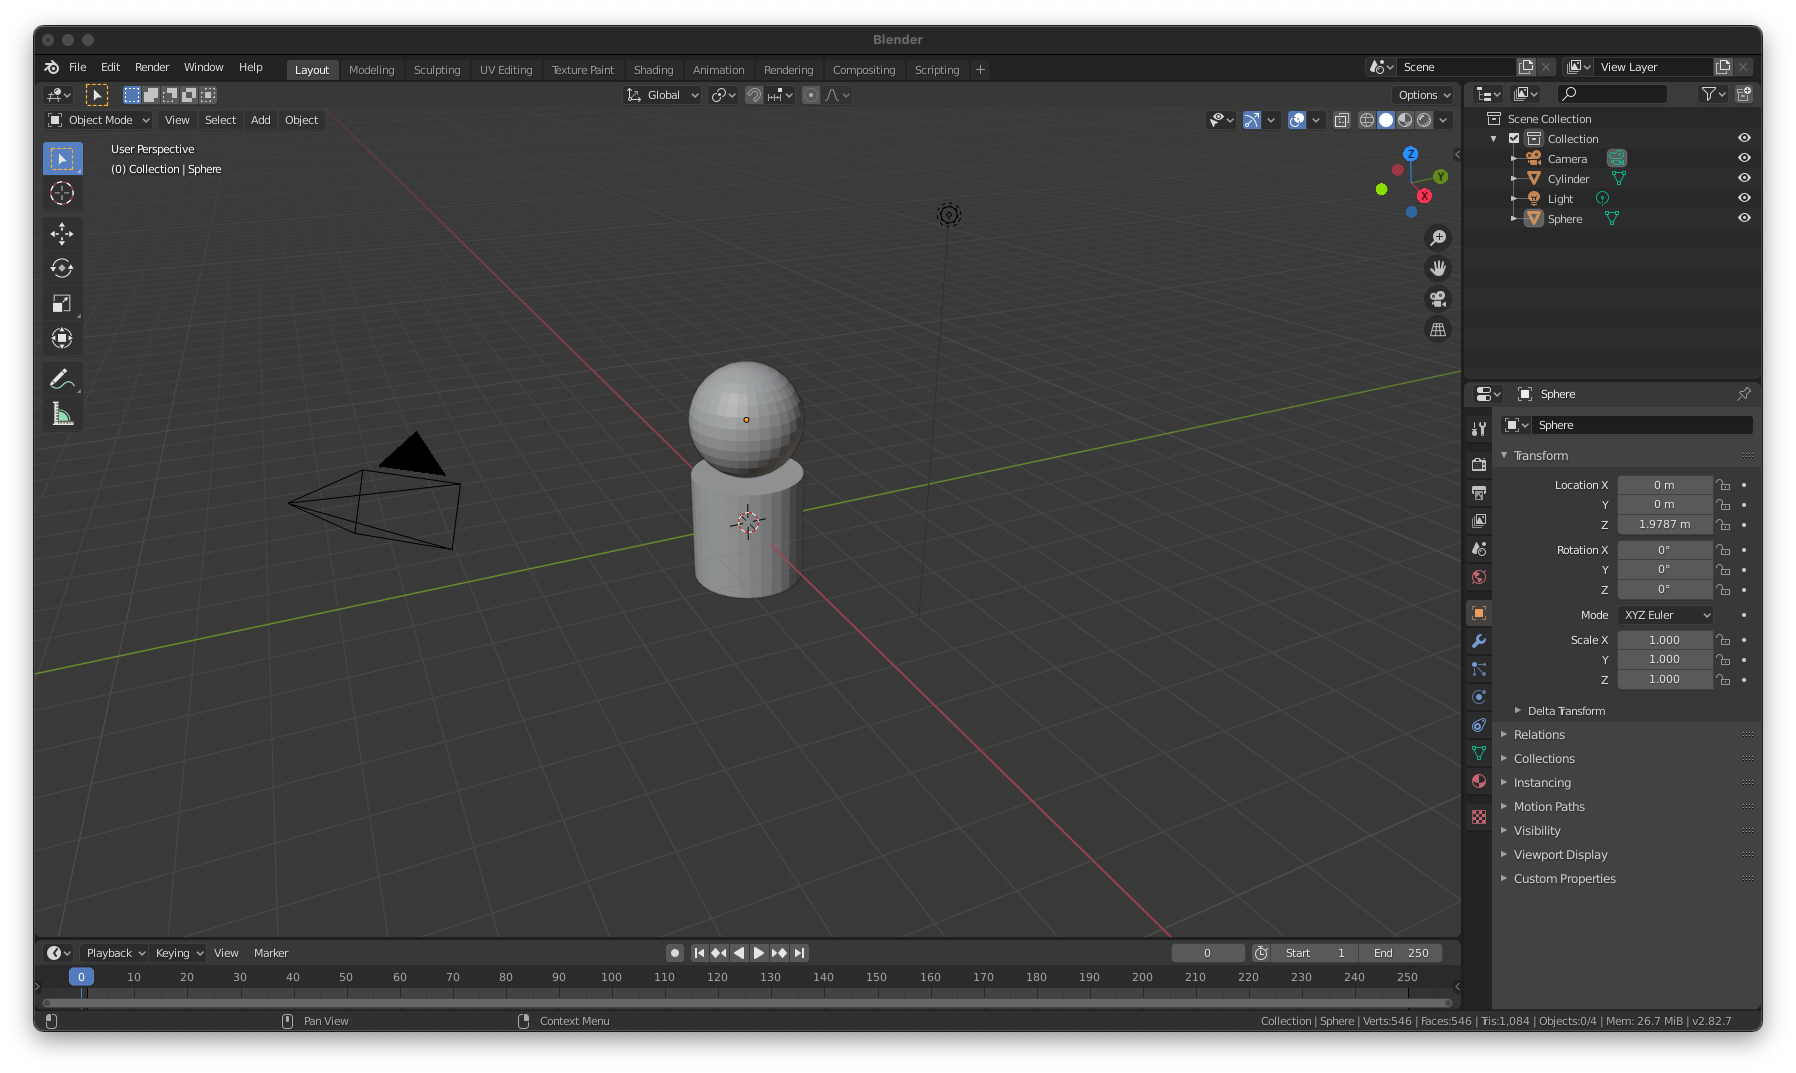
\includegraphics[width=1\textwidth]{bilder/blender.png}

	\caption[Blender-Arbeitsbereich]{Blender bietet verschiedene Perspektiven und Werkzeuge, um komplexe Gebilde präzise zu modellieren. }

	\label{fig:blender}
\end{figure}

Blender bietet neben 3D-Navigations-Schaltflächen eine große Zahl an Werkzeugen, mit denen Modelle erstellt und bearbeitet werden können, sowie vorgefertigte Formen. Objekte können unter anderem verschoben, verzerrt, geteilt und zusammengefügt werden.

Zudem gibt es Szenen-Objekte, die besondere Funktionen besitzen. Neben der Kamera, deren Position und Ausrichtung für das Ergebnisbild entscheidend ist, können auch verschiedenartige Lichtquellen und Spiegel in der Szene platziert werden, die in die Berechnung des Endergebnisses einbezogen werden. Zudem können Animationseffekte wie Feuer, Wasser und Wind erzeugt werden.
\pagebreak

Es wurde ein Blender-Python-Script entwickelt (s.~\hyperref[blenderpy]{Anhang 3}), um Bilder automatisiert erstellen zu lassen. Das Skript exportiert das Ergebnis als Waveform-OBJ und als JPEG-Bilddatei.

Zunächst werden drei Zufallswerte für die Breite, Höhe und Tiefe jeweils der Tischplatte sowie der Tischbeine ermittelt. Für den Abstand der Tischbeine von der Tischkante wird ein weiterer Zufallswert berechnet. Anschließend werden Blender-Standard-Würfel so in der Szene platziert und anhand der Zufallswerte verformt, dass die Form eines Tisches entsteht.

Die Tischform wird mit einer Textur versehen, damit eine Holzoptik entsteht.

Die Objekte werden anschließend ausgewählt, um fünfmal um den entsprechenden Anteil einer Umdrehung ($\pi/5$) gedreht zu werden. Dies geschieht in einer Schleife. Nach jeder Drehung wird eine Bilddatei gespeichert.

Der gesamte Vorgang wird selbst in einer Schleife durchgeführt, sodass nach einer Ausführung 50 verschiedene Tische generiert und zu jedem Tisch fünf Bilddateien, also insgesamt 250 Bilddateien, gespeichert wurden.


\section{Anwendung herkömmlicher Shader}
\label{sec:shader}
In der Computergrafik wird die Darstellung der Oberfläche eines Objekts durch die drei Faktoren Material, Textur und Ausleuchtung bestimmt. Material ist die Grundfarbe der Oberfläche. Es legt fest, wie das sichtbare Spektrum des Lichts von der Oberfläche des Objekts reflektiert wird. Ein Material legt außerdem fest, ob die Oberfläche matt oder metallisch erscheint. Es kann entsprechend der drei Farbschemas RGB, HSV oder Hex dargestellt werden. Wie die Farbe in jedem Schema erscheint ist auch von einem Alpha-Wert, welcher für die Menge der Transparenz steht, abhängig. Textur sind die physischen Charakteristiken der Oberfläche, und Ausleuchtung ist die Hintergrundbeleuchtung oder Licht, welches von Lichtern (Lampen) emittiert wird. \cite{blain2020blender}

Texturen definieren das physische Erscheinungsbild einer Oberfläche, also etwa wie glatt oder uneben diese erscheint, oder ihre Struktur, welche die visuelle Wahrnehumg der physischen Beschaffenheit des Objekts definiert. Diese Definition bestimmt, woraus die Oberfläche besteht, wie Holz, Ziegelsteine, Wasser und so weiter. Texturen werden durch Algorithmen generiert, wie sie in Blender integriert sind (prozedurale Texturen) oder aus Bilddateien (Bildtexturen). \cite{blain2020blender}

Shader definieren die Interaktion des Lichts mit der Oberfläche des Objekts. Dabei können Shader aus einem oder mehreren BSDFs (Bidirectional Scattering Distribution Function) bestehen, die wiederum von Mix-und Add-Shadern in der Zusammensetzung gemischt werden. Polygonobjekte sind anfangs immer ungeglättet, das heißt, dass beim Rendern oder in der schattierten Ansicht zunächst immer die einzelnen Flächen zu sehen sind, aus denen sich das Objekt zusammensetzt. Eine mögliche, wenn auch in Sachen Renderzeit und Speicherverbrauch ungünstige Methode wäre, einfach das Objekt so weit in kleinere Flächen zu unterteilen, dass beim Rendern eine Fläche pro Pixel gerendert wird. In der praktischen Arbeit verwendet man deshalb einen Trick, bei dem die Übergänge zwischen den einzelnen Flächen ``glattgerechnet'' werden. Übliche Verfahren hier sind das Gouraud oder Phong Shading. \cite{wartmann2014blender}

Die Qualität eines Bildes hängt direkt von der Effektivität des Shading-Algorithmus ab, der wiederum von der Modellierungsmethode des Objektes abhängt. Zwei wesentliche Methoden der Objektbeschreibung werden häufig verwendet, nämlich Oberflächendefinition mittels mathematischer Gleichungen und Oberflächenapproximation durch Mosaike aus polygonalen Flächen. \cite{phong1975shading}


\section{Hyperparameter}
\label{sec:hyperparams}
Die Pix2Pix-Referenzimplementierung ist bereits für die Übersetzung von Skizzen in Fotos eingestellt. Für das Training waren anfangs $40000$ Trainingsschritte vorgesehen. Je nach Größe des Trainingssets werden also mehrere Wiederholungen mit demselben Trainingsset durchgeführt, um zufriedenstellende Ergebnisse zu erzielen. Nach Abschluss der Experimente könnte die Anzahl der Trainingsschritte auf $30000$ reduziert werden, um die Dauer des Trainings und die Ergebnisse zu optimieren. Dies ist aber wiederum abhängig von der Größe des Trainingssets. Es war auch im Sinne des Experiments, das Modell einige Tausend Schritte mehr durchführen zu lassen als für das optimale Resultat erforderlich gewesen wären.

Die Eingabebilder sind 256x256 Pixel groß und besitzen einen Farbkanal für Graustufen. Sie werden am Anfang des Trainingsprozesses durch sogenanntes Jittering augmentiert. Dabei werden die Bilder zuerst auf 286x286 Pixel vergrößert und anschließend auf einen zufälligen 256x256 Pixel großer Ausschnitt wieder verkleinert. Änderungen an diesen Pixelgrößen haben im Experiment keine nennenswerte Verbesserung bewirkt.

Der Adam Optimierer \cite{kingma2017adam} erhält für die Learning-Rate den Wert $0,0002$. Das Momentum ist auf $0,9$ voreingestellt. Diese beiden Werte beinflussen die Lerngeschwindigkeit und sind in begrenztem Maße anpassbar, sind aber bereits für meinen Zwecke optimal eingestellt.

\section{Performancebeobachtungen}
\label{sec:performance}
Das Training umfasst sinnvollerweise 15000 bis 40000 Iterationen. Die Implementierung sieht vor, dass alle 1000 Iterationen ein Zwischenergebnis in Form dreier Bilder gespeichert wird. Das zu speichernde Beispiel kann dabei zufällig gewählt werden, oder es kann der Fortschritt eines einzelnen Input-Target-Paars über die Iterationen hinweg gezeichnet werden.

\begin{figure}[h]
	\centering
	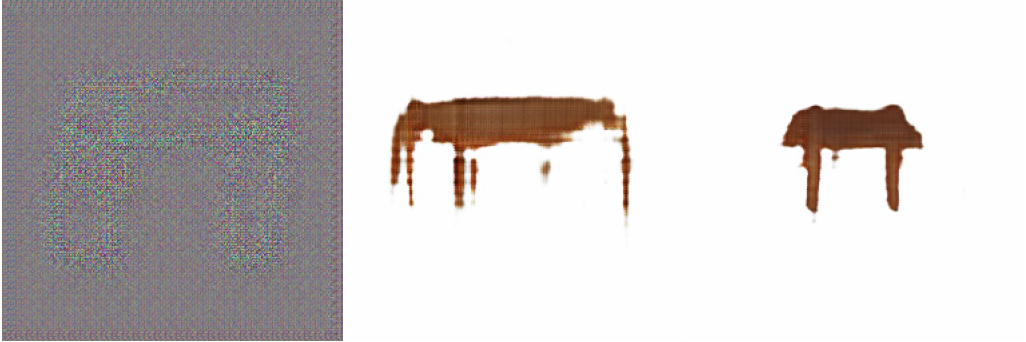
\includegraphics[width=1.0\textwidth]{bilder/pix2pix_progress/progress_tables.png}
	\caption[Lernfortschritt am Beispiel von Tischen 1]{Generierte Bilder von Tischen vor dem Training, nach 1000 Iterationen und nach 2000 Iterationen}
	\label{fig:pix2pixprogress1}
\end{figure}

\begin{figure}[h]
  \centering
	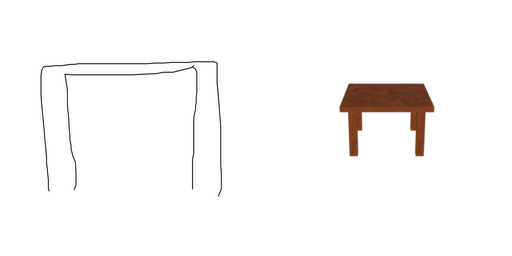
\includegraphics[width=0.8\textwidth]{bilder/pix2pix_progress/394_input.png}
  \caption[Quadratischer Tisch]{Ein Beispiel eines Tisches, dessen Textur und Form gelernt werden soll}
  \label{fig:trainingexample}
\end{figure}

Abbildung \ref{fig:trainingexample} zeigt beispielhaft eine handgezeichnete Skizze eines Tisches und das erwartete Ergebnis. In diesem Beispiel wird versucht, aus einem vermutlich quadratischen, gänzlich von der Seite gezeichneten Tisch einen quadratischen, von leicht schräg oben betrachteten texturierten Tisch zu generieren.

In Abbildung \ref{fig:pix2pixprogress1} ist zu erkennen, wie sich innerhalb 2000 Iterationen die Qualität der generierten Bilder von zufälligem Bildrauschen zu einem bereits als Tisch erkennbaren Objekt verbessert. In diesem Trainingsset befanden sich unterschiedlich hohe, unterschiedlich breite und auch im Raum unterschiedlich ausgerichtete Tische. Es ist auch zu erkennen, dass aus der handgezeichneten Skizze bereits ein quadratischer Tisch generiert wird.

Nicht korrekt werden in dieser Phase des Trainings die geraden Linien der Zielbilder erzielt. Auch die Anzahl der Tischbeine stimmt noch nicht.

\begin{figure}[h]
	\centering
	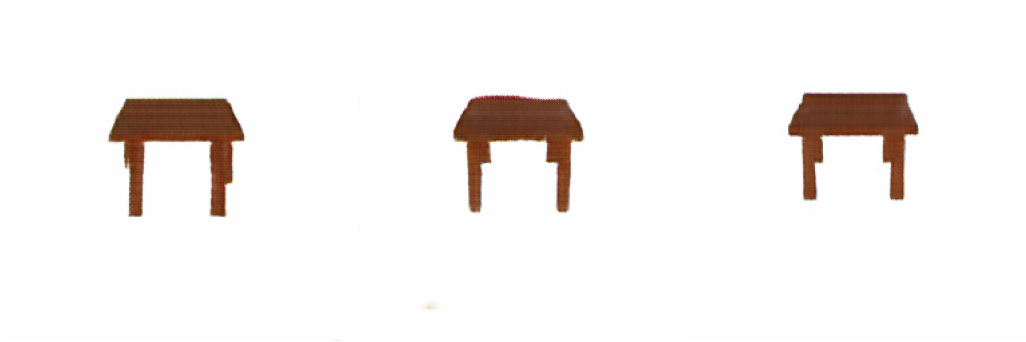
\includegraphics[width=1.0\textwidth]{bilder/pix2pix_progress/progress_tables2.png}
	\caption[Lernfortschritt am Beispiel von Tischen 2]{Generierte Bilder von Tischen nach 10000, 15000 und 20000 Iterationen}
	\label{fig:pix2pixprogress2}
\end{figure}

In Abbildung \ref{fig:pix2pixprogress2} wird der Lernerfolg während der zweiten Hälfte von insgesamt 20000 Iterationen gezeigt. Zunächst ist das Ergebnis noch stellenweise unscharf und die Länge der Tischbeine ist ungleich. Die Kanten sind bereits gerade. Nach 15000 Iterationen ist zu erkennen, dass häufigeres Trainieren nicht unbedingt bessere Ergebnisse bringt. Nach Abschluss des Trainings sieht der generierte Tisch aus wie die Vorgabe im Trainingsset.

Das Modell hat Form und Farbe verschiedener Tische gelernt. Auch die Unregelmäßigkeiten in der Färbung der Tische wurde erlernt. Das ist die zweite Frage, die in dieser Arbeit zu beantworten war. Es ist einem künstlichen neuronalen Netz also möglich Texturen zu erlernen.

\begin{figure}[h]
	\centering
	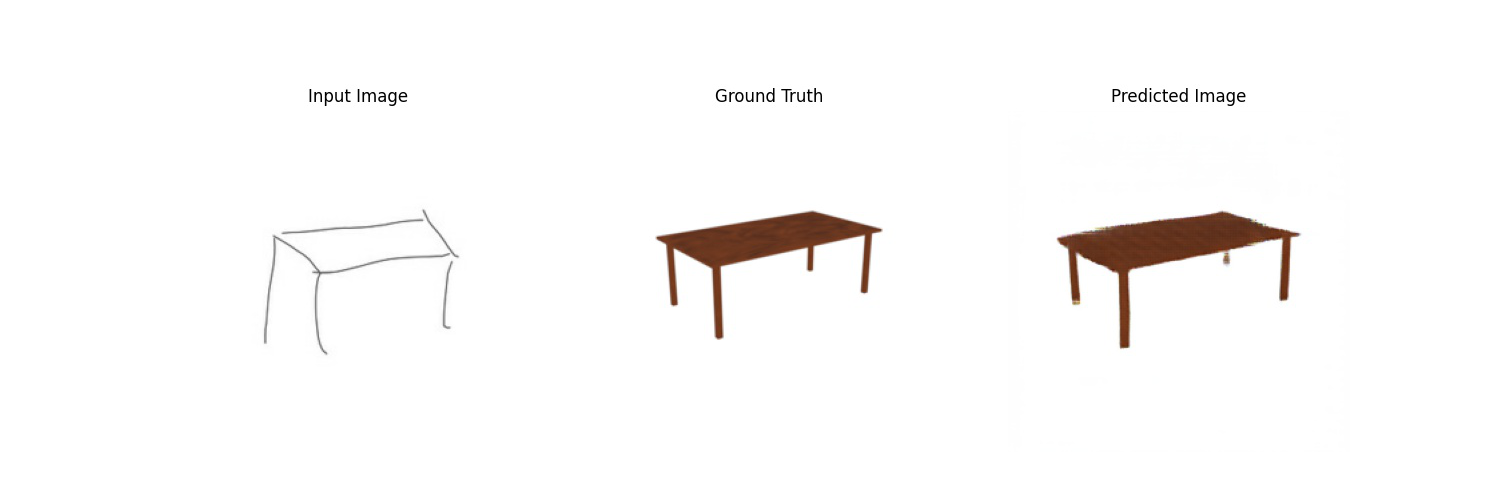
\includegraphics[width=0.875\textwidth]{bilder/pix2pix_progress/table_result_orientation1.png}
  \caption[Tisch korrekt ausgerichtet]{Korrekt ausgerichteter Tisch mit unregelmäßigen Kanten}
  \label{fig:pix2pixorientation1}

	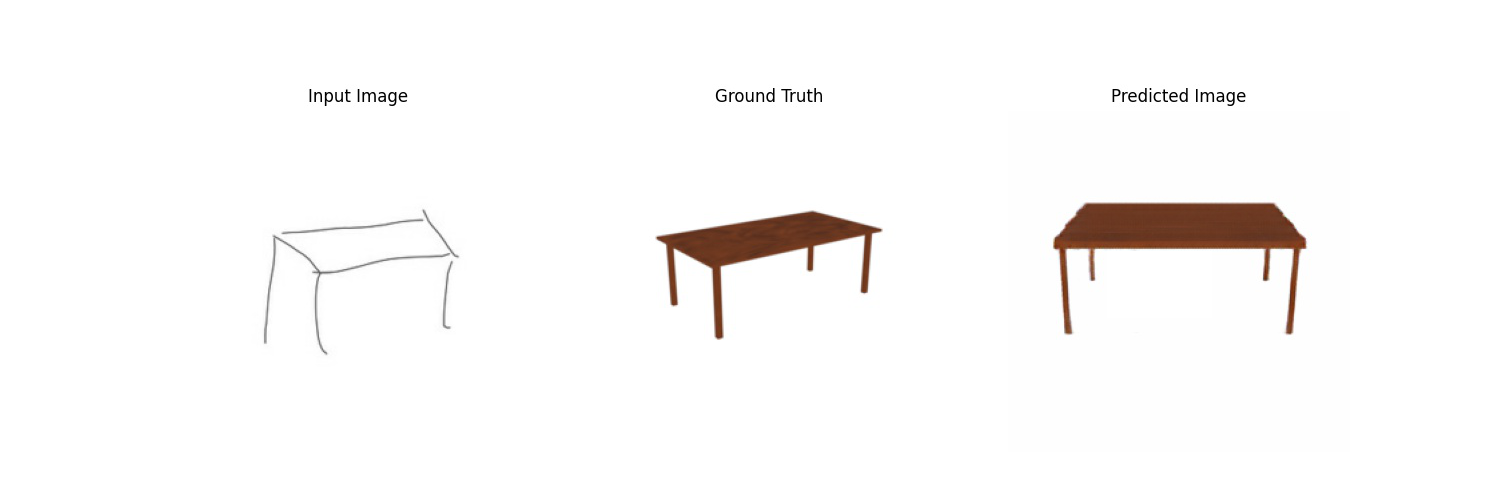
\includegraphics[width=0.875\textwidth]{bilder/pix2pix_progress/table_result_orientation2.png}
	\caption[Tisch mit geraden Kanten]{Tisch mit geraden Kanten, aber falscher Ausrichtung}
	\label{fig:pix2pixorientation2}
\end{figure}

In Abbildung \ref{fig:pix2pixorientation1} ist ein Beispielergebnis aus einem Trainingsdurchlauf mit 262 Tischen zu sehen. Der Tisch ist so im Raum ausgerichtet wie im Zielbild vorgesehen. Die Form ist aber ungleichmäßig und das Bild teilweise verschwommen.

Abbildung \ref{fig:pix2pixorientation2} zeigt eines der Ergebnisse aus einem Trainingsdurchlauf mit 960 verschiedenen Tischen. Der Tisch hat gerade und scharfe Kanten, die Tischplatte ist aber parallel zum unteren und oberen Bildrand.

Der Vergleich zeigt, wieviel Bedeutung der Datenqualität des Trainingssets zukommt. Das kleinere Trainingsset war eine Teilmenge des größeren, enthielt aber anteilig mehr schräg im Raum ausgerichtete Tische. Obwohl das mit 960 Bildern trainierte Modell also dieselben schräg ausgerichteten Tische verwendete, generiert es vorzugsweise Bilder von gerade ausgerichteten Tischen.

\begin{figure}[h]
	\centering
	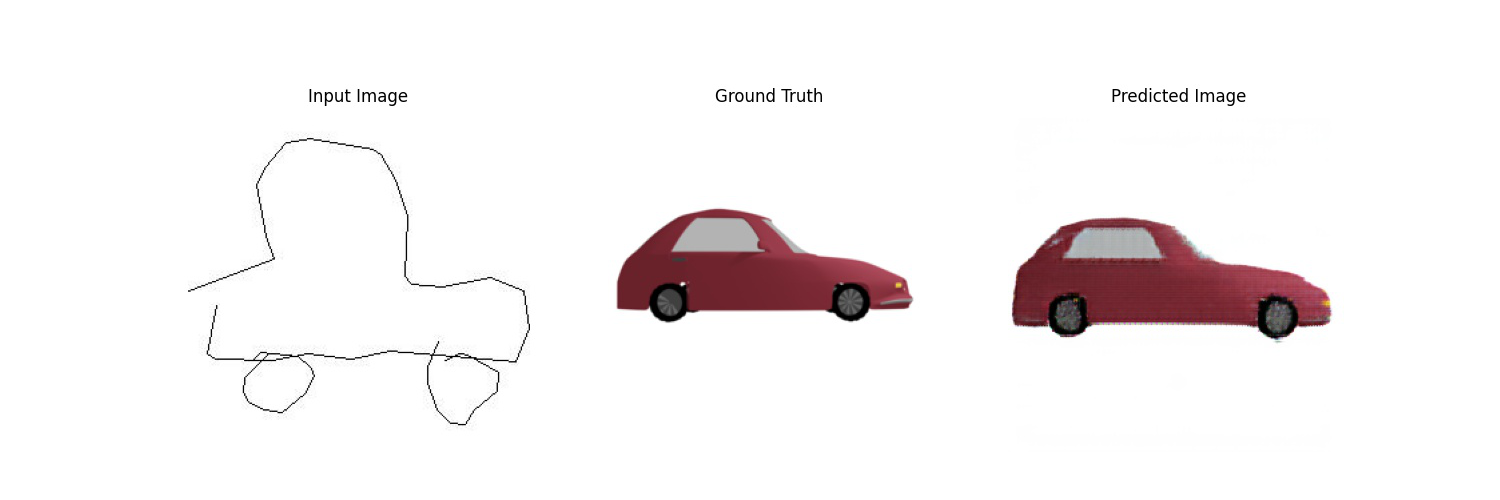
\includegraphics[width=0.9\textwidth]{bilder/pix2pix_progress/car_small.png}
	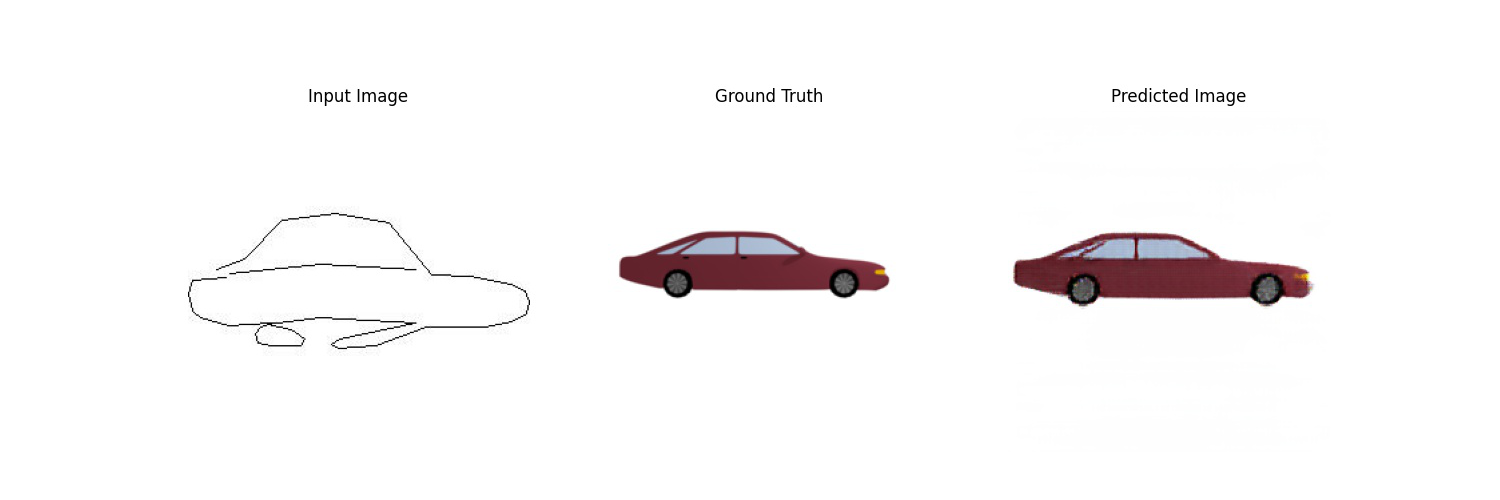
\includegraphics[width=0.9\textwidth]{bilder/pix2pix_progress/car_limo.png}
	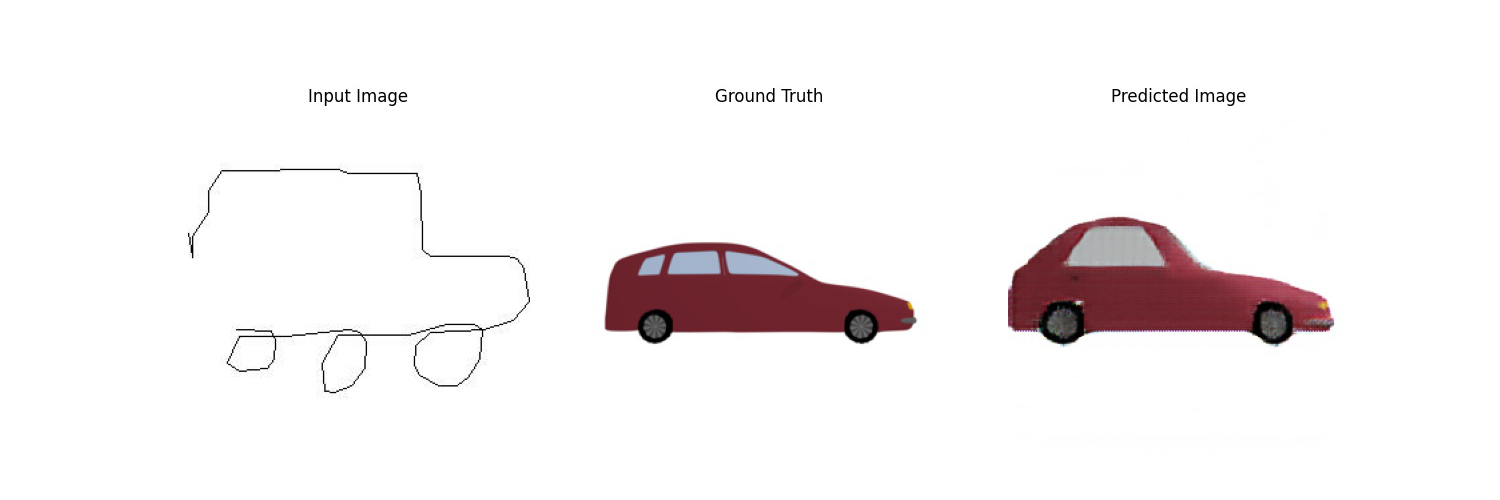
\includegraphics[width=0.9\textwidth]{bilder/pix2pix_progress/car_kombi.png}
	\caption[Generierte Autos]{Beispiele für generierete Autos}
	\label{fig:pix2pixcars}
\end{figure}

Fahrzeuge, wie in Abbildung \ref{fig:pix2pixcars}, sind eine vergleichbar schwierige Aufgabe für ein künstliches neuronales Netz. Aufgrund der Vielfalt an möglichen Fahrzeugen, für die der Begriff ``Auto'' (englisch ``Car'') stehen kann, unterscheiden sich die Zeichnungen im Quick!Draw-Dataset sehr stark und sind nur schwer zu sortieren und Zielbildern zuzuordnen.

Genauso aufwendig ist es, verschiedene Fahrzeuge zu modellieren, um sie als Zielbilder zu verwenden. Anders als bei vielen Eigenschaften von Tischen, wie die Stärke der Tischplatte und der Tischbeine, lassen sich die Unterschiede von PKWs nicht genauso gut durch Zufallszahlen beschreiben. Auch sind die Autos fast ausschließlich in der Seitenansicht gezeichnet, sodass automatisch in verschiedenen Perspektiven gerenderte Blendermodelle der Fahrzeuge fast nicht nutzbar sind.

Die Handskizzen stellen hauptsächlich PKWs dar und wurden deshalb nur in die drei Kategorien Limousine, Kleinwagen und Kombi unterteilt und entsprechenden Zielbildern zugewiesen.

In den Abbildungen sind unterschiedlich gute Resultate zu sehen. Für einen praktischen Einsatzzweck, wie zum Beispiel ein Lehrmittel in einer Fahrschule, wäre dieses Modell bestenfalls als Grundlage für weiterführende Trainings geeignet.

Die Trainingsergebnisse habe ich hauptsächlich durch Ansicht beurteilt. In Tensorflow wird der Trainingsfortschritt in Zahlen als Diagramm dargestellt. Das verwendete Skript erstellt drei Diagramme für den Generator und ein Diagramm für den Discriminator. Generator und Discriminator werden gleichzeitig trainiert. Der Verlust des Discriminators nimmt im Verlauf des Trainings ab. Nach $20000$ bis $30000$ Iterationen ist die Abnahme weniger stark.

Der Discriminator wird auf das vom Generator erstellte Bild und auf das Zielbild angewendet. Der Gesamtverlust des Discriminators wird aus diesen beiden Ergebnissen gebildet und bezeichnet den Erfolg beziehungsweise Misserfolg des Discriminators, das durch den Generator erstellte Bild als solches von einem Zielbild zu unterscheiden.

Wie bei cGANs üblich wird der Gesamtverlust des Generators ebenfalls aus zwei verschiedenen Ergebnissen berechnet. Die beiden Faktoren sind in Abbildung \ref{fig:pix2pixprogress4} als gen\_l1\_loss und gen\_gan\_loss bezeichnet.

Einerseits wird der pixelweise Unterschied zwischen dem generierten Bild und dem Zielbild als Verlustindikator herangezogen. Dieser Wert wird 100fach gewichtet, hat also einen entsprechend größeren Einfluss auf das Gesamtergebnis. Er nimmt im Laufe des Trainings sichtbar ab.

Das GAN-Loss berücksichtigt das Ergebnis des Discriminators, also wie gut dieser das generierte Bild von einem Zielbild unterscheiden konnte. Im Diagramm ist zu erkennen, dass sich der Verlust im Verlauf des Trainings sogar erhöht. Die Erklärung dafür ist der immer geringere Verlust des Discriminators, der dadurch generierte Bilder und Zielbilder besser voneinander unterscheiden kann.

\begin{figure}[h]
	\centering
	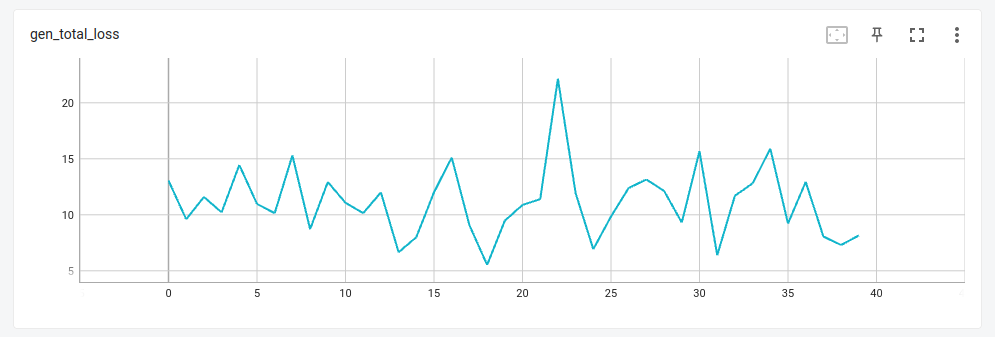
\includegraphics[width=0.925\textwidth]{bilder/pix2pix_progress/gen_total_loss.png}
	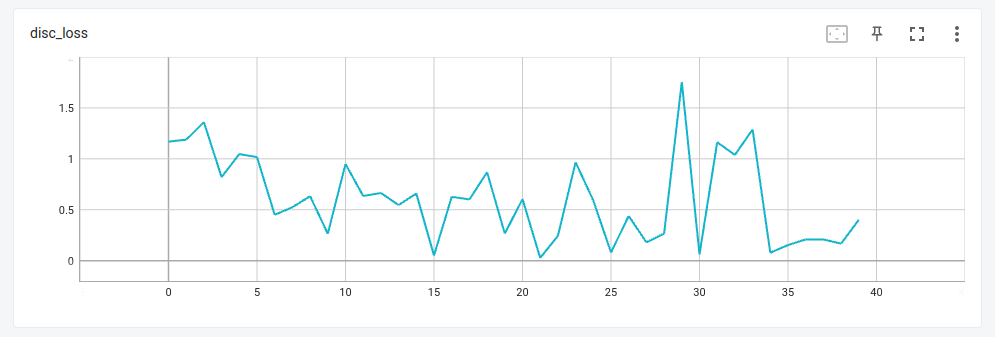
\includegraphics[width=0.925\textwidth]{bilder/pix2pix_progress/disc_loss.png}
	\caption[Verlustdiagramm 1]{Die Tensorboard-Diagramme des Gesamtverlusts jeweils für Generator (gen\_total\_loss) und für Discriminator (disc\_loss) }
	\label{fig:pix2pixprogress3}
	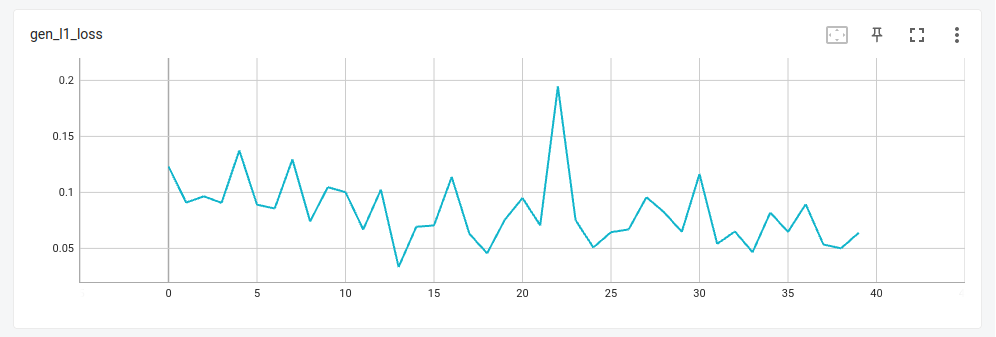
\includegraphics[width=0.925\textwidth]{bilder/pix2pix_progress/gen_l1_loss.png}
	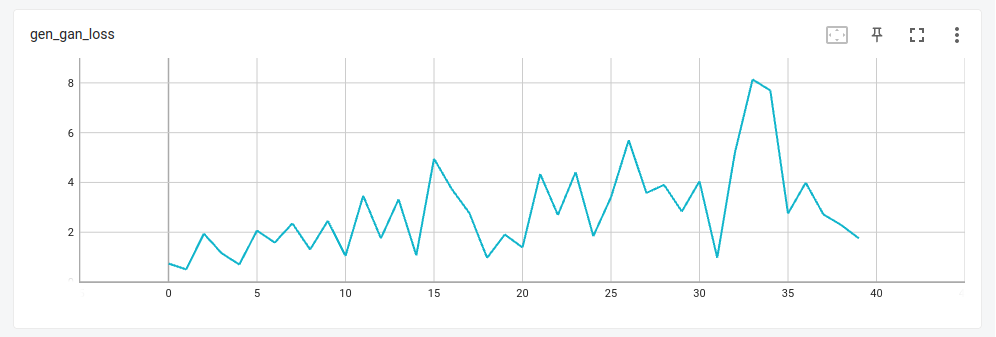
\includegraphics[width=0.925\textwidth]{bilder/pix2pix_progress/gen_gan_loss.png}
	\caption[Verlustdiagramm 2]{Die Tensorboard-Diagramme der Generator-Verluste}
	\label{fig:pix2pixprogress4}
\end{figure}

\clearpage

In den Diagrammen ist der Verlauf eines Trainings über $40000$ Iterationen abgebildet. Im Trainingsset befanden sich 262 verschiedene Tische und das Testset enthielt sechs Tische. Trotz des relativ kleinen Trainingssets wurde ein visuell überzeugendes Resultat erzielt. Nach $20000$ bis $30000$ verbesserte sich der Lernerfolg nicht mehr wesentlich. Ein Versuch mit $80000$ Iterationen hat gezeigt, dass eine viel größere Anzahl Iterationen das Resultat eher verschlechtert.

\chapter{Diskussion}
\label{sec:conclusion}
Bildgenerierung mittels künstlichen neuronalen Netzen wurde bereits in verschiedenen Experimenten und mit teilweise sehr guten Ergebnissen durchgeführt und dokumentiert. Es können Bildteile aus den umliegenden Bildinformationen neu generiert werden, wie es mit Fotobearbeitungssoftware möglich ist.

Seit einiger Zeit sind Handschrifterkennungs-Algorithmen verbreitet. Eine Variante der Bildgenerierung ist deren Umkehr, indem zum Beispiel aus einstelligen Zahlen handschriftlich aussehende Ziffern generiert werden. Außerdem kann der Gesamteindruck eines vorhandenen Bildes, auch durch Verwendung eines weiteren Bildes, verändert und auf diese Art ein neues Bild generiert werden.

Die Arbeit mit künstlichen neuronalen Netzen hat gezeigt, dass ein Großteil des Aufwands aus der Erhebung und Vorbereitung der Daten besteht. Geeignete Eingabebilder mussten entweder gesammelt oder selbst erstellt werden. Durch Automatisierung konnte der Erstellungsprozess verkürzt werden, machte aber immer noch einen erheblichen Anteil der Arbeit aus. Sowohl gesammelte als auch selbst erstellte Bilder eignen sich nicht ausnahmslos für den gewählten Zweck. Es war deshalb weiterhin erforderlich, die Bilder händisch zu sortieren. Anschließend war noch jeweils die Zuweisung einer Handskizze zu einem Ergebnisbild erforderlich, die ebenfalls manuell erfolgen musste.

Das Training des Modells ist ein weiterer aufwendiger Prozess. Im Laufe eines Trainingdurchlaufes eines künstlichen neuronalen Netzes zeichnet sich bereits ein Endergebnis ab. Es ist daher möglich, anhand weniger Zwischenergebnisse schwerwiegende Fehler zu bemerken und den Durchlauf von vorn zu beginnen. Das Endergebnis ist selbstverständlich erst nach Abschluss des Trainings sichtbar. Wenn es darum geht herauszufinden, wieviele Durchläufe für ein perfektes Ergebnis erforderlich sind, kann es erforderlich sein das Modell mehrere Male hintereinander auf dasselbe Ergebnis zu trainieren.

Künstliche neuronale Netze sind mathematische Konstrukte. Zunächst ist es deshalb erforderlich, die Fachbegriffe der entsprechenden Literatur zu kennen. Die wissenschaftlichen Texte liegen hauptsächlichich auf Englisch vor, sodass man die Begriffe sinnvollerweise auf Deutsch und auf Englisch lernt. Das künstliche neuronale Netz selbst wird als eine Struktur aus Tensoren dargestellt.

Die Algorithmen des maschinellen Lernens berechnen üblicherweise aus der Eingabe mehrere weitere Schichten aus Tensoren. Die Dimensionalität der Tensoren ändert sich auf jeder weiteren Schicht. Einige Algorithmenklassen, wie zum Beispiel die U-Net-Architektur, sind benannt nach der Art, auf die sich die Dimensionalität der Tensoren ändert.

Für diese Arbeit waren die Generative Adversarial Networks besonders interssant. Mit ihnen werden zwei lernende Komponenten gegeneinander angesetzt. Eine von ihnen lernt die eigentliche Aufgabe zu erfüllen. Die zweite Komponente wird darauf trainiert, die Ergebnisse der ersten zu bewerten und Feedback zu den Ergebnissen zu geben.

Die für maschinelles Lernen erforderlichen Berechnungen können auf handelsüblichen PCs ausgeführt werden. Sie sind aber sehr umfangreich, sodass sich unterstützende Hardware günstig auswirkt. Bei Cloud-Angeboten wie Google Colab und Amazon SageMaker, die auf Implementierungen dieser Art spezialisiert sind, können Algorithmen auf Enterprise-Grade-Hardware ausgeführt werden.

Aber auch Grafikkarten für Spiele-PCs sind durch parallele Tensoroperationen für maschinelles Lernen um ein Vielfaches besser geeignet als die CPU. Für diesen Zweck existiert speziell hergestellte Treibersoftware. Die Parallelisierungssoftware für NVIDIA-Grafikkarten heißt CUDA. Auf die Treiber aufbauend wurden und werden Programmierschnittstellen für verschiedene Programmiersprachen entwickelt.

Eine der weit verbreitetsten Machine-Learning-Programmierschnittstellen ist Tensorflow für Python, die auch für diese Arbeit verwendet wurde. Die Einrichtung auf einem Desktopcomputer ist teilweise umständlich, aber für Tensorflow und CUDA gut dokumentiert. Es gibt Anleitungen für Ubuntu Linux. Die Verwendung der Programmierschnittstelle ist ebenfalls gut dokumentiert. Den in dieser Arbeit verwendeten Machine-Learning-Algorithmus Image-To-Image-Translation ist in der Beispielsektion auf tensorflow.org\footnote{\href{https://tensorflow.org}{https://tensorflow.org}} zu finden.

Das Modell muss immer wieder von vorn trainiert werden, bevor erste brauchbare Ergebnisse erzielt werden. Grundsätzlich gilt, dass die Menge der Eingabedaten so groß wie möglich sein sollte, damit ein Lernprozess erfolgreich sein kann. Trotzdem sind weitere Eigenschaften des Datasets wichtig. An dem Beispiel der Tische wurde deutlich, dass die Perspektive, also die Ausrichtung der Tische im Raum, nur bei einem ausreichenden Anteil an schräg ausgerichteten Beispielen erlernt wird. Dafür kann es sogar sinnvoll sein, die Gesamtgröße des Datasets zu reduzieren, damit alle Varianten in genügend großen Anteilen im Dataset vorhanden sind.

Die Anzahl der Trainingsdurchläufe ist eine der wichtigsten Größen beim maschinellen Lernen. In Klassifizierungsalgorithmen gibt es das Phänomen des Overfittings, das die Erfolgsrate bei den Klassifizierungen negativ beeinflusst. Dieses Problem gibt es bei der Bildgenerierung zunächst nicht, solange wie beschrieben die Beispiele im Dataset ausgewogen sind. Trotzdem ist diese Größe selbstverständlich für die Untersuchung und den Einsatz eines ML-Modells aufgrund des Zeitaufwands relevant.

Während der Versuchreihen wurde erkennbar, welche Bildinformationen durch ein künstliches neuronales Netz erlernt werden können, um eigenständig Bilder zu generieren. Die Möglichkeit Bilder überhaupt mittels künstlichen neuronalen Netzen generieren zu können war die erste und wichtigste Frage, die mit dieser Arbeit beantwortet werden sollte. Die Frage wurde recherchiert, und es standen mehrere Methoden zur Auswahl.

Die konkreten Einsatzmöglichkeiten für Deep Learning sind, abgesehen von einigen nicht praxisorientierten Anwendungsbeispielen, ausschließlich in wissenschaftlichen Artikeln zu finden. Diese Artikel setzen beim Leser üblicherweise ein Verständnis der Grundlagen voraus und verweisen bestenfalls auf vorherige Arbeiten. Für die grundlegenden Prinzipien des maschinellen Lernens und verschiedene Arten von künstlichen neuronalen Netzen wie CNNs und RNNs gibt es Literatur in Form von Büchern. Die Bücher liegen größtenteils in englischer Sprache vor. Es gibt nur wenig deutsche Literatur. Die wissenschaftlichen Artikel zu dem Thema gibt es ausschließlich auf Englisch.

Die besonders vielseitig einsetzbare Methode namens Image-To-Image-Translation ist in der Lage fehlende Bildinformationen zu generieren, neu zu generieren oder jeweils den umgekehrten Vorgang durchzuführen. Zum Beispiel können Schwarz-Weiß-Bilder koloriert, Luftaufnahmen in Karten übersetzt oder Straßenbilder nur aus Informationen zu Verkehrsteilnehmern und Straßenverläufen generiert werden, beziehungsweise jeweils auch umgekehrt. Mit dieser Bildübersetzung ist es auch möglich, aus handgezeichneten Gesichtern Portraitfotos oder Portraits, die wie von einem Künstler gemalt aussehen, zu generieren. Das kommt dem Generieren von Bildern aus handgezeichneten Skizzen am nächsten, anhand dessen in dieser Arbeit diese Fähigkeit künstlicher neuronaler Netze gezeigt werden sollte.

In dem Artikel zu Image-To-Image-Translation wird die zugrundliegende Situation beschrieben, in der von einem Eingabebild zum Ausgabebild Pixel für Pixel übersetzt wird. Dies trifft etwa auf die Übersetzung eines Umrisses auf ein Foto desselben Objekts zu. Der Algorithmus lernt dann dem Objekt eine Textur zu geben. Die Frage, ob ein künstiches neuronales Netz lernen kann Texturen zu generieren, war die zweite Frage, die in dieser Arbeit zu beantworten war. Die Ergebnisse zu den entsprechenden Versuchen waren größtenteils sehr gut. Die Holztextur für die Tische und auch der Helligkeitsverlauf der brennenden Kerzen wurden sehr gut gelernt.

Eine Schwäche bei der Generierung von Bildern aus Handskizzen scheinen die unregelmäßigen und fast nie geraden Umrisse der skizzierten Objekte zu sein. Auch in den Trainingsergebnissen mit vielen einwandfrei generierten Bildern fanden sich häufig noch Bilder mit unsauberen Stellen. Besonders die scharfen Übergänge wie zum Beispiel vom Rad eines Autos zur Karosserie oder einfach die Kanten des Objektes waren oft verschwommen. Die Flammen auf den Zielbildern der Kerzen waren von einen Lichtschein umgeben. Der wurde zwar gelernt, aber das Ergebnis ist optisch nicht ansprechend. Tische waren im Trainingsset immer mit genau vier Beinen vorgegeben. Auf den Ergebnisbildern waren oft andere Anzahlen der Tischbeine zu sehen.

Einige der Schwierigkeiten könnten gemindert werden, indem die Eingabedaten noch stärker vorbereitet werden. Zum Beispiel könnten die Maße und die Ausrichtung in den Skizzen der Tische ermittelt werden und diese Werte für die Generierung der Ergebnisbilder verwendet werden. Der Lichtschein um die Flamme einer Kerze könnte auch auf eine andere Weise als durch ein künstliches neuronales Netz dem Ergebnisbild nachträglich hinzugefügt werden.

Die praktische Anwendung dieser Methode in einem Anwendungsprogramm zur Innenraumgestaltung ist sehr gut vorstellbar. Dafür müssten nur noch einige weitere Objekte zur Auswahl stehen, wie Möbelstücke, Lampen, Teppiche und so weiter. Ein Classifier wäre dann vorteilhaft, um die Generierung der richtigen Einrichtungsgegenstände sicherzustellen. Auch eine Anwendung in einem Smartboard für die Verkehrserziehung oder in einer Fahrschule ist nach den in dieser Arbeit gezeigten Ergebnissen vorstellbar. Um Fahrzeuge aus verschiedenen Perspektiven generieren zu können sind entsprechende Eingabebilder, sowohl Ergebnisbilder als auch handgezeichnete Skizzen, zu erstellen.
